% Options for packages loaded elsewhere
\PassOptionsToPackage{unicode}{hyperref}
\PassOptionsToPackage{hyphens}{url}
%
\documentclass[
]{article}
\usepackage{amsmath,amssymb}
\usepackage{lmodern}
\usepackage{iftex}
\ifPDFTeX
  \usepackage[T1]{fontenc}
  \usepackage[utf8]{inputenc}
  \usepackage{textcomp} % provide euro and other symbols
\else % if luatex or xetex
  \usepackage{unicode-math}
  \defaultfontfeatures{Scale=MatchLowercase}
  \defaultfontfeatures[\rmfamily]{Ligatures=TeX,Scale=1}
\fi
% Use upquote if available, for straight quotes in verbatim environments
\IfFileExists{upquote.sty}{\usepackage{upquote}}{}
\IfFileExists{microtype.sty}{% use microtype if available
  \usepackage[]{microtype}
  \UseMicrotypeSet[protrusion]{basicmath} % disable protrusion for tt fonts
}{}
\makeatletter
\@ifundefined{KOMAClassName}{% if non-KOMA class
  \IfFileExists{parskip.sty}{%
    \usepackage{parskip}
  }{% else
    \setlength{\parindent}{0pt}
    \setlength{\parskip}{6pt plus 2pt minus 1pt}}
}{% if KOMA class
  \KOMAoptions{parskip=half}}
\makeatother
\usepackage{xcolor}
\usepackage[margin=1in]{geometry}
\usepackage{color}
\usepackage{fancyvrb}
\newcommand{\VerbBar}{|}
\newcommand{\VERB}{\Verb[commandchars=\\\{\}]}
\DefineVerbatimEnvironment{Highlighting}{Verbatim}{commandchars=\\\{\}}
% Add ',fontsize=\small' for more characters per line
\usepackage{framed}
\definecolor{shadecolor}{RGB}{248,248,248}
\newenvironment{Shaded}{\begin{snugshade}}{\end{snugshade}}
\newcommand{\AlertTok}[1]{\textcolor[rgb]{0.94,0.16,0.16}{#1}}
\newcommand{\AnnotationTok}[1]{\textcolor[rgb]{0.56,0.35,0.01}{\textbf{\textit{#1}}}}
\newcommand{\AttributeTok}[1]{\textcolor[rgb]{0.77,0.63,0.00}{#1}}
\newcommand{\BaseNTok}[1]{\textcolor[rgb]{0.00,0.00,0.81}{#1}}
\newcommand{\BuiltInTok}[1]{#1}
\newcommand{\CharTok}[1]{\textcolor[rgb]{0.31,0.60,0.02}{#1}}
\newcommand{\CommentTok}[1]{\textcolor[rgb]{0.56,0.35,0.01}{\textit{#1}}}
\newcommand{\CommentVarTok}[1]{\textcolor[rgb]{0.56,0.35,0.01}{\textbf{\textit{#1}}}}
\newcommand{\ConstantTok}[1]{\textcolor[rgb]{0.00,0.00,0.00}{#1}}
\newcommand{\ControlFlowTok}[1]{\textcolor[rgb]{0.13,0.29,0.53}{\textbf{#1}}}
\newcommand{\DataTypeTok}[1]{\textcolor[rgb]{0.13,0.29,0.53}{#1}}
\newcommand{\DecValTok}[1]{\textcolor[rgb]{0.00,0.00,0.81}{#1}}
\newcommand{\DocumentationTok}[1]{\textcolor[rgb]{0.56,0.35,0.01}{\textbf{\textit{#1}}}}
\newcommand{\ErrorTok}[1]{\textcolor[rgb]{0.64,0.00,0.00}{\textbf{#1}}}
\newcommand{\ExtensionTok}[1]{#1}
\newcommand{\FloatTok}[1]{\textcolor[rgb]{0.00,0.00,0.81}{#1}}
\newcommand{\FunctionTok}[1]{\textcolor[rgb]{0.00,0.00,0.00}{#1}}
\newcommand{\ImportTok}[1]{#1}
\newcommand{\InformationTok}[1]{\textcolor[rgb]{0.56,0.35,0.01}{\textbf{\textit{#1}}}}
\newcommand{\KeywordTok}[1]{\textcolor[rgb]{0.13,0.29,0.53}{\textbf{#1}}}
\newcommand{\NormalTok}[1]{#1}
\newcommand{\OperatorTok}[1]{\textcolor[rgb]{0.81,0.36,0.00}{\textbf{#1}}}
\newcommand{\OtherTok}[1]{\textcolor[rgb]{0.56,0.35,0.01}{#1}}
\newcommand{\PreprocessorTok}[1]{\textcolor[rgb]{0.56,0.35,0.01}{\textit{#1}}}
\newcommand{\RegionMarkerTok}[1]{#1}
\newcommand{\SpecialCharTok}[1]{\textcolor[rgb]{0.00,0.00,0.00}{#1}}
\newcommand{\SpecialStringTok}[1]{\textcolor[rgb]{0.31,0.60,0.02}{#1}}
\newcommand{\StringTok}[1]{\textcolor[rgb]{0.31,0.60,0.02}{#1}}
\newcommand{\VariableTok}[1]{\textcolor[rgb]{0.00,0.00,0.00}{#1}}
\newcommand{\VerbatimStringTok}[1]{\textcolor[rgb]{0.31,0.60,0.02}{#1}}
\newcommand{\WarningTok}[1]{\textcolor[rgb]{0.56,0.35,0.01}{\textbf{\textit{#1}}}}
\usepackage{longtable,booktabs,array}
\usepackage{calc} % for calculating minipage widths
% Correct order of tables after \paragraph or \subparagraph
\usepackage{etoolbox}
\makeatletter
\patchcmd\longtable{\par}{\if@noskipsec\mbox{}\fi\par}{}{}
\makeatother
% Allow footnotes in longtable head/foot
\IfFileExists{footnotehyper.sty}{\usepackage{footnotehyper}}{\usepackage{footnote}}
\makesavenoteenv{longtable}
\usepackage{graphicx}
\makeatletter
\def\maxwidth{\ifdim\Gin@nat@width>\linewidth\linewidth\else\Gin@nat@width\fi}
\def\maxheight{\ifdim\Gin@nat@height>\textheight\textheight\else\Gin@nat@height\fi}
\makeatother
% Scale images if necessary, so that they will not overflow the page
% margins by default, and it is still possible to overwrite the defaults
% using explicit options in \includegraphics[width, height, ...]{}
\setkeys{Gin}{width=\maxwidth,height=\maxheight,keepaspectratio}
% Set default figure placement to htbp
\makeatletter
\def\fps@figure{htbp}
\makeatother
\setlength{\emergencystretch}{3em} % prevent overfull lines
\providecommand{\tightlist}{%
  \setlength{\itemsep}{0pt}\setlength{\parskip}{0pt}}
\setcounter{secnumdepth}{5}
\newlength{\cslhangindent}
\setlength{\cslhangindent}{1.5em}
\newlength{\csllabelwidth}
\setlength{\csllabelwidth}{3em}
\newlength{\cslentryspacingunit} % times entry-spacing
\setlength{\cslentryspacingunit}{\parskip}
\newenvironment{CSLReferences}[2] % #1 hanging-ident, #2 entry spacing
 {% don't indent paragraphs
  \setlength{\parindent}{0pt}
  % turn on hanging indent if param 1 is 1
  \ifodd #1
  \let\oldpar\par
  \def\par{\hangindent=\cslhangindent\oldpar}
  \fi
  % set entry spacing
  \setlength{\parskip}{#2\cslentryspacingunit}
 }%
 {}
\usepackage{calc}
\newcommand{\CSLBlock}[1]{#1\hfill\break}
\newcommand{\CSLLeftMargin}[1]{\parbox[t]{\csllabelwidth}{#1}}
\newcommand{\CSLRightInline}[1]{\parbox[t]{\linewidth - \csllabelwidth}{#1}\break}
\newcommand{\CSLIndent}[1]{\hspace{\cslhangindent}#1}
\ifLuaTeX
  \usepackage{selnolig}  % disable illegal ligatures
\fi
\IfFileExists{bookmark.sty}{\usepackage{bookmark}}{\usepackage{hyperref}}
\IfFileExists{xurl.sty}{\usepackage{xurl}}{} % add URL line breaks if available
\urlstyle{same} % disable monospaced font for URLs
\hypersetup{
  pdftitle={Sources, behavior and fate of nutrients and their implications for the formulation of aquafeeds and nutrient management tailored for aquaponic systems},
  pdfauthor={Anıl Axel Tellbüscher},
  hidelinks,
  pdfcreator={LaTeX via pandoc}}

\title{Sources, behavior and fate of nutrients and their implications for the formulation of aquafeeds and nutrient management tailored for aquaponic systems}
\author{Anıl Axel Tellbüscher}
\date{}

\begin{document}
\maketitle

{
\setcounter{tocdepth}{2}
\tableofcontents
}
\hypertarget{introduction}{%
\section{Introduction}\label{introduction}}

Aquaponics is a hybrid food production system, coupling aquaculture and soilless horticulture (hydroponics). In comparison with uncoupled, independent systems, advocates of the aquaponics principle with an aquaculture background claim that added value is created by preventing the release of aquaculture wastes into the environment but converting them into edible yield instead (Turnsek et al. 2020). Furthermore, it was found that there is no significant difference in the yield of several leafy greens such as lettuce, spinach, basil, dill, coriander, parsley, rook and even fruiting plants such as tomato that can be achieved in aquaponic versus hydroponic systems (Lennard and Goddek 2019; \textbf{Atique2022?}; \textbf{Anderson2017?}; Maucieri et al. 2019; \textbf{Suhl2016?}; Pantanella et al. 2012). This is noteworthy against the background that nutrient deficiencies are frequently reported when comparing the nutrient concentrations in aquaponic systems with those usually targeted in hydroponics (Lunda et al. 2019; Robaina et al. 2019; \textbf{Graber2009?}; Bittsánszky et al. 2016). On the other hand, the complexity of the system adds extra costs to aquaponics. Achieving similar yield is thus seen as insufficient to render aquaponics competitive under present circumstances when compared with conventional hydroponics (Quagrainie et al. 2017). Interestingly, aquaponics seems to offer the potential to reach even higher yields than in hydroponics if certain nutrients are amended. This was described for lettuce (Monsees et al. 2019; Delaide et al. 2016), basil (Rodgers et al. 2022) and tomato (\textbf{Roosta2013?}). However, a simple ``off-the-shelf'' solution for the management of plant nutrients that is as simple as the commercially available and fine-tuned plant fertilizers used in hydroponics is lacking. The development of a specific feed for aquaponic systems, hereinafter denoted as aquafeed, is thought to be such a solution (\textbf{Lennard2017?}; Eck, Körner, and Jijakli 2019).

As of today, the essentiality of 15 elements that are usually grouped into macro- and micronutrients, according to their abundance in plant tissues, is established for higher plants. Elements classified as macronutrients are carbon (C), hydrogen (H), oxygen (O), nitrogen (N), phosphorus (P), potassium (K), calcium (Ca), magnesium (Mg), and sulfur (S), while the micronutrients comprise iron (Fe), manganese (Mn), copper (Cu), zinc (Zn), molybdenum (Mo), and boron (B) (Marschner 2012). The essentiality of nickel (Ni) and chloride (Cl) is currently under discussion (Mengel et al. 2001).

In aquaponic systems, the aquafeed and the source water are considered as main sources of nutrients (Eck, Körner, and Jijakli 2019). In addition, alkalinity supplements can play an important role in the supply of nutrients (Rakocy, Masser, and Losordo 2006). These sources vary in their contribution to the total daily nutrient input, depending on the species reared and the location of the facility.

Aquafeeds are usually considered as of greatest importance in terms of nutrient input into aquaponic systems (Robaina et al. 2019). Though, data about the inclusion rates of nutrients relevant for plants in commercial aquafeeds is scarce because these compounds are either not essential for aquatic animals or can be taken up from water via the gills in sufficient quantities. These nutrients are thus usually not considered during feed formulation (Lall 2002).
An aquafeed can vary in its nutrient composition due to slight changes in its raw material composition caused by fluctuations in feed ingredient availability and market prices. While feed manufacturers allow variations of crucial nutrients such as the crude protein (CP) inclusion rate only within tight limits, this is not the case for other nutrients that are disregarded in the formulation process. However, data about the ranges of microminerals in commercial aquafeeds is not available in literature.

When discussing aquafeeds as nutrient input, it is important to consider their route of excretion, as shown in \textbf{Figure XXX} @ref(fig:pathway\_digestion). Only dissolved nutrients are available for plant uptake. After ingestion by the cultivated animal, the indigestible mass fraction is excreted in form of solid matter. The digestible mass fraction is eventually utilized to sustain the basal metabolism, somatic growth and reproductive activity of the animal and the metabolic end products are then excreted in form of dissolved matter via the gills and the urinary system (\textbf{Evans2005?}; Hardy 2002).

\begin{figure}
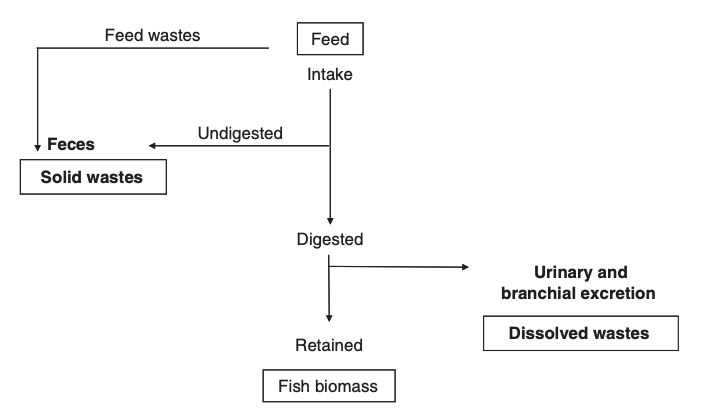
\includegraphics[width=9.78in]{images/2010_Bureau} \caption{A simple graphical representation of nutrient flows and excretion patterns in aquatic animals (from Bureau and Hua, 2010).}(\#fig:pathway_digestion)
\end{figure}

N that is, for the most part, present as CP in aquafeeds, is usually well-digestible, with the apparent digestibility coefficient (ADC) of feed ingredients usually being above 70\% and on average approximately 90\% (International Aquaculture Feed Formulation Database (IAFFD) 2021; Guillaume et al. 2001). The excretion of N as end product of the protein and amino acid catabolism takes place in form of ammonia and, to a small extent, urea. The predominant excretory site are the gills, followed by renal excretion (Dabrowski and Guderley 2002).

A less digestible nutrient is P with ADC estimates ranging from 70\% to 40\% and a resulting excretion of 30\% to 60\% of the supply (Lall 2002; Sugiura 2018). Especially plant ingredients in aquafeeds can cause low ADC if they are rich in phytic acid. Phytic acid is poorly digestible and can furthermore reduce the digestibility of minerals in the feed. This might also explain contradictory information in literature with reported renal excretion rates of 90\% of the total excreta (\textbf{Tomiyama1956?}) in contrast to estimates of 28\% of excretion taking place in dissolved form and 30\% to 64\% excreted as particulate P (Dabrowski and Guderley 2002).

In terms of digestibility, information about the remaining plant nutrients is scarce. Variability of ADC among different feed ingredients was shown in Atlantic salmon (\emph{Salmo salar}) for Ca, Mg, Fe, Mn and Zn, with an ADC ranging between 30\% to 50\% (Sugiura et al. 1998).

Excretion of the earth alkaline metals Ca and Mg takes primarily place in dissolved form via the gills and urine (Lall 2002; Oikari and Rankin 1985). Mn, in contrast, is mostly excreted in solid form as feces, while the renal excretion was found to be negligible (Lall 2002). Cu is predominantly excreted via the bile (Bury, Walker, and Glover 2003). Excess dietary Cu is not taken up but excreted as feces. Thus the Cu inclusion rate in aquafeeds is reduced to minimize its release into the environment (Lall 2002). Zn is mostly excreted renally and via the gills (Lall 2002).

Tap water can vary in its composition, depending on its origin such as surface or groundwater. The extent of the variability of terrestrial waters in their chemical composition is shown in \textbf{FIGURE XXX}. Wheathering of rock, ion exchange, redox reactions and the buildup of biomass are the main processes that are affecting the concentrations of the shown compounds (Stumm 1981). The highest variability can be found in anionic compounds such as nitrate (\(\text{NO}_{3}^{-}\)) and sulfate (\(\text{SO}_{4}^{2-}\)) and the cationic alkaline earth metals \(\text{Ca}^{2+}\) and \(\text{Mg}^{2+}\) that are covering a concentration range of approximately two orders of magnitude.

Due to its low water demand, aquaponics is generally seen as food production system suitable for urban areas or arid regions (Kloas et al. 2015; Joyce et al. 2019). Establishing an aquaponic system in these regions comes with limited access to water sources such as well water or rivers and lakes. Rainwater, on the other hand, would require large storage capacities. Tap water is thus assumed to be the most important water source.

The quality of tap water is usually rigidly regulated by the authorities. In Europe, the Drinking Water Directive is defining maximum allowable concentrations (MAC), setting threshold concentrations for several substances that could affect the consumers' health. Other MAC such as for Fe are of technical nature, where exceeding the limit could indicate for instance damages in the municipal water installation (Council of the European Union 2020). \textbf{TABLE XXX} summarizes MAC of plant nutrients that are regulated by the Drinking Water Directive. Even though the source water is seen as of minor importance in terms of nutrient influx, it was found that a comparably large proportion of some plant nutrients such as Ca, Mg and S, can originate from source water (Delaide et al. 2017).

\textbf{Average plant nutrient composition found in trout, salmon, and eel grower feeds (Tacon and Silva 1983) and maximum allowable concentrations (MAC) of substances considered as plant nutrients defined by the EU Drinking Water Directive (Council of the European Union 2020).}

\begin{longtable}[]{@{}lll@{}}
\toprule()
Nutrient & Aquafeeds & Tap water (limit) \\
\midrule()
\endhead
\(\text{NO}_{3}^{-}\) & - & 50 mg L\(^{-1}\) \\
\(\text{NO}_{2}^{-}\) & - & 0.5 mg L\(^{-1}\) \\
\(\text{NH}_{4}^{+}\) & - & 0.5 mg L\(^{-1}\) \\
TIN & \(64 \text{ g kg}^{-1}\) \footnote{Calculated based on an aquafeed with 40\% CP (dry matter base) and the Kjeldahl factor 6.25.} & 50 mg L\(^{-1}\) \footnote{Calculated as {[}TIN{]} = {[}\(\text{NH}_{4}^{+}\){]} + {[}\(\text{NO}_{2}^{-}\){]} + {[}\(\text{NO}_{3}^{-}\){]}.} \\
P & 13.26 g kg\(^{-1}\) & no MAC \\
K & 9.83 g kg\(^{-1}\) & no MAC \\
Ca & 17.75 g kg\(^{-1}\) & no MAC \\
Mg & 2.13 g kg\(^{-1}\) & no MAC \\
\(\text{SO}_{4}^{2-}\) & & 250 mg L\(^{-1}\) \\
Fe & 229 mg kg\(^{-1}\) & 200 µg L\(^{-1}\) \\
Mn & 96 mg kg\(^{-1}\) & 50 µg L\(^{-1}\) \\
Cu & 14 mg kg\(^{-1}\) & 2 mg L\(^{-1}\) \\
Zn & 163 mg kg\(^{-1}\) & no MAC \\
Ni & 3 mg kg\(^{-1}\) & 20 µg L\(^{-1}\) \\
\bottomrule()
\end{longtable}

\begin{figure}
\centering
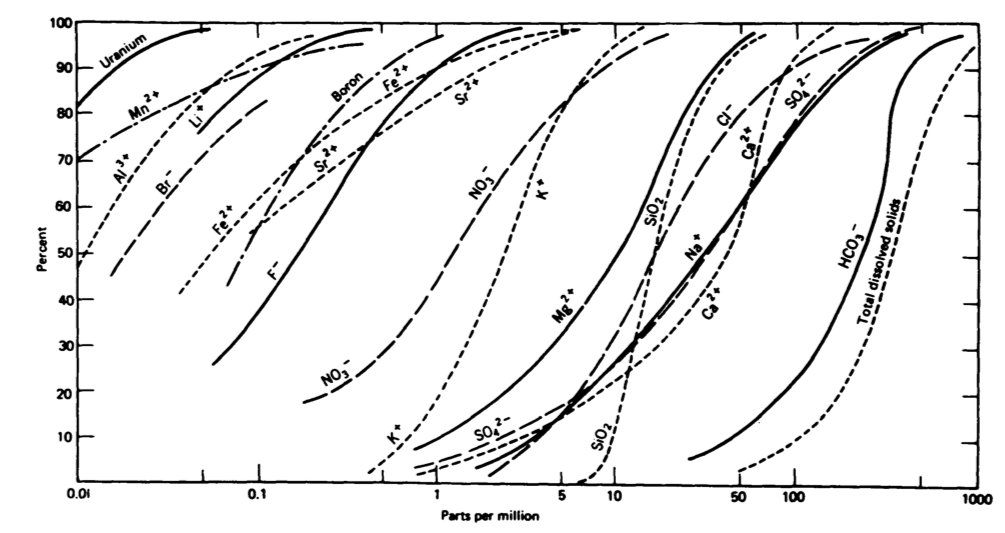
\includegraphics{images/Stumm_Morgan_Aquatic_Chemistry_p873.png}
\caption{Cumulative frequency distribution of chemical compounds in terrestrial water. X-axis: logarithmic concentration of compounds. 1 ppm = 1 mg/L. Y-axis: Percentage of sampling points (from Stumm and Morgan, 1996).}
\end{figure}

Lastly, the third continuous nutrient input are alkalinity supplements that are used to maintain a stable pH in the system (Timmons 2010). The activity of nitrifying bacteria in the biofilter releases three moles of protons (H\(^{+}\)) per mole of ammonia (NH\(_{3}\)) that is converted to NO\(_{3}^{-}\). This leads to a decrease in pH over time and consequently to a decrease in the activity of the nitrifyers (Ward, Arp, and Klotz 2011). Thus, the released H\(^{+}\) has to be neutralized to maintain a stable pH and ensure both high nitrification performance and the welfare of the fish stock. For this purpose, several Na-based alkalinity supplements such as sodium hydrogen carbonate (baking soda, NaHCO\(_{3}\)) are commonly used in aquaculture due to their high and rapid solubility and a comparably cheap price. However, high daily Na inputs should be avoided due to its phytotoxicity at high concentrations (Maathuis, Ahmad, and Patishtan 2014). Therefore, several other supplements based on K or Ca are used in aquaponics.
\textbf{TABLE XXX} summarises some supplements, their properties and prices. These substances come with the advantage of providing additional plant nutrients while increasing the pH.

\textbf{Properties and prices of some Na based alkalinity supplements used in aquaculture and their K and Ca based alternatives for aquaponics (adapted from Bisogni and Timmons, 1994). Prices from \url{https://www.alibaba.com} (accessed January 14th, 2023). All chemicals food grade and with a minimum order quantity of one kilogram. Reported is the cheapest sales price.}

\begin{longtable}[]{@{}
  >{\raggedright\arraybackslash}p{(\columnwidth - 8\tabcolsep) * \real{0.2000}}
  >{\raggedright\arraybackslash}p{(\columnwidth - 8\tabcolsep) * \real{0.2000}}
  >{\raggedright\arraybackslash}p{(\columnwidth - 8\tabcolsep) * \real{0.2000}}
  >{\raggedright\arraybackslash}p{(\columnwidth - 8\tabcolsep) * \real{0.2000}}
  >{\raggedright\arraybackslash}p{(\columnwidth - 8\tabcolsep) * \real{0.2000}}@{}}
\toprule()
\begin{minipage}[b]{\linewidth}\raggedright
Chemical Formula
\end{minipage} & \begin{minipage}[b]{\linewidth}\raggedright
Common Name
\end{minipage} & \begin{minipage}[b]{\linewidth}\raggedright
Solubility
\end{minipage} & \begin{minipage}[b]{\linewidth}\raggedright
Solubilization rate
\end{minipage} & \begin{minipage}[b]{\linewidth}\raggedright
Price
\end{minipage} \\
\midrule()
\endhead
\(\text{NaOH}\) & sodium hydroxide & high & rapid & \(\approx 0.30 \text{ EUR kg}^{-1}\) \\
\(\text{Na}_{2}\text{CO}_{3}\) & sodium carbonate, soda ash & high & rapid & \(\approx 0.20 \text{ EUR kg}^{-1}\) \\
\(\text{NaHCO}_{3}\) & sodium bicarbonate, baking soda & high & rapid & \(\approx 0.01 \text{ EUR kg}^{-1}\) \\
\(\text{KOH}\) & potassium hydroxide & high & rapid & \(\approx 0.60 \text{ EUR kg}^{-1}\) \\
\(\text{K}_{2}\text{CO}_{3}\) & potassium carbonate & high & rapid & \(\approx 0.50 \text{ EUR kg}^{-1}\) \\
\(\text{KHCO}_{3}\) & potassium bicarbonate & high & rapid & \(\approx 0.50 \text{ EUR kg}^{-1}\) \\
\(\text{CaCO}_{3}\) & calcium carbonate, calcite & moderate & moderate & \(\approx 0.13 \text{ EUR kg}^{-1}\) \\
\(\text{CaO}\) & slaked lime & high & moderate & \(\approx 0.10 \text{ EUR kg}^{-1}\) \\
\(\text{Ca(OH)}_{2}\) & calcium hydroxide, hydrated lime & high & moderate & \(\approx 0.25 \text{ EUR kg}^{-1}\) \\
\(\text{CaMg(CO}_{3})_{2}\) & dolomite & moderate & slow & \(\approx 0.10 \text{ EUR kg}^{-1}\) \\
\bottomrule()
\end{longtable}

\hypertarget{chemical-reactions-affecting-plant-nutrient-availability}{%
\subsection{Chemical reactions affecting plant nutrient availability}\label{chemical-reactions-affecting-plant-nutrient-availability}}

Hydroponics literature highlights that an understanding of aquatic chemistry is crucial for successful nutrient management (Sambo et al. 2019). The prerequisite for plant nutrients to be available for plant uptake via the roots is that they must be present in dissolved form. However, the concentration of dissolved substances underlies physico-chemical constrains. In hydroponics, these constraints are well-described as they have to be taken into account when intending to formulate cost-efficient fertilizers (De Rijck and Schrevens 1999b).
The most important reactions that are determining the concentration of plant nutrients in water are dissolution-precipitation, acid-base, and complex formation reactions (Sambo et al. 2019). The following description of the named reactions intends to give a very brief introduction into their underlying mechanisms and their relevance for nutrient management. Describing these reactions in greater detail is out of scope of this manuscript. Further information can be obtained by consulting the dedicated literature (Jensen 2003; Stumm 1981).

Dissolution of a salt occurs if its ionic compounds are present in solution below a concentration denoting the saturation concentration of the same or another salt containing these ions. The saturation concentration of a salt can be described using solubility product constants \(K_{sp}\), which are the product of the concentration of the cation(s) and the anion(s) at saturation concentration, as shown in \textbf{equation XXX}, with square brackets denoting for molar concentrations.

\[
K_{sp} = [cation^{n+}]^{m} \cdot [anion^{m-}]^{n}
\]

\(K_{sp}\) is either determined empirically or derived from thermodynamic data. The saturation concentration \(S\) of the salt can eventually be calculated by rearranging \textbf{equation XXX} as shown in \textbf{equation XXX}.

\[
S = \sqrt[m+n]{\frac{K_{sp}}{m^{m} \cdot n^{n}}}
\]

If the concentrations of the cation(s) and anion(s) in solution are known, it is possible to calculate the ion product \(Q\) analogously to the calculation of \(K_{sp}\) as shown in \textbf{equation XXX}, substituting \([cation]\) and \([anion]\) by the corresponding empirical data.

\[
Q = [cation^{n+}]^{m} \cdot [anion^{m-}]^{n}
\]

\(K_{sp}\) can now be compared with \(Q\) to evaluate whether the solution is saturated or not by calculating the saturation index \(U\) as shown in \textbf{equation XX}. If the saturation concentration is exceeded (\(Q > K_{sp}\) and \(\log{\frac{Q}{K}} > 0\)), precipitation occurs.

\[
U = \log{\frac{Q}{K_{sp}}}
\]

The formation of a salt can also be seen as the result of a neutralisation reaction. For instance, the reaction of phosphoric acid (H\(_{3}\)PO\(_{4}\)) with sodium hydroxide (NaOH) can be written in a simplified way as

H\(_{3}\)PO\(_{4}\) + NaOH \textless-\textgreater{} NaH\(_{2}\)PO\(_{4}\) + H\(_{2}\)O

, yielding sodium dihydrogen phosphate (NaH\(_{2}\)PO\(_{4}\)) as product. A salt thus consists of the conjugated weak base (H\(_{2}\)PO\(_{4}^{-}\)) and acid (Na\(^{+}\)) of the strong acid (H\(_{3}\)PO\(_{4}\)) and base (NaOH) that led to its formation.

When a salt dissolves, or its strong acids or bases are introduced into the system, they undergo acid-base reactions with water. As an example, the reactions of trihydrogen phosphate (H\(_{3}\)PO\(_{4}\)), commonly termed phosphoric acid, with water are

H\(_{3}\)PO\(_{4}\) + H\(_{2}\)O \textless-\textgreater{} H\(_{2}\)PO\(_{4}^{-}\) + H\(_{3}\)O\(^{+}\) \(K_{a1} = 10^{2.1}\)

H\(_{2}\)PO\(_{4}^{-}\) + H\(_{2}\)O \textless-\textgreater{} HPO\(_{4}^{2-}\) + H\(_{3}\)O\(^{+}\) \(K_{a2} = 10^{7.2}\)

HPO\(_{4}^{2-}\) + H\(_{2}\)O \textless-\textgreater{} PO\(_{4}^{3-}\) + H\(_{3}\)O\(^{+}\) \(K_{a3} = 10^{12.0}\)

The reactions show that phosphate in aqueous solution is present in four forms, which there are H\(_{3}\)PO\(_{4}\), H\(_{2}\)PO\(_{4}^{-}\), HPO\(_{4}^{2-}\) and PO\(_{4}^{3-}\), that differ in their degree of protonation. These forms are the so-called species. The extent to which the described dissociation reactions (the removal of H\(^{+}\)) occurs depends on the pH of the system and can be mathematically described by a characteristic equilibrium constant \(K_{a}\) for each reaction step (Jensen 2003).
The species differ in their chemical behavior, with PO\(_{4}^{3-}\) being known for forming precipitates if, for instance, both PO\(_{4}^{3-}\) and Ca\(^{2+}\) ions are present in solution and \(Q > K_{sp}\). This could be avoided by complex formation reactions where a chelating agent, forms a complex molecule which is ``hidden'' and thus excluded from precipitation. Complex molecules are formed especially with cations of transition metal and they can lead to concentrations of these metals that are exceeding their saturation concentrations by three to four orders of magnitude (Jensen 2003).

\hypertarget{differences-between-hydroponic-and-aquaponic-systems}{%
\subsection{Differences between hydroponic and aquaponic systems}\label{differences-between-hydroponic-and-aquaponic-systems}}

An understanding of the effects and constraints that are resulting from the described reactions is crucial for successful nutrient management in both hydroponic and aquaponic systems to ensure that nutrients that are introduced into the system are in fact present in a plant-available form. With respect to typical hydroponic conditions, these effects were exhaustively described (De Rijck and Schrevens 1997, 1998b, 1998a, 1999b). However, no such work has been conducted for aquaponics.
Overall, the two main differences described between hydroponic and aquaponic systems are 1) the pH and 2) the concentration of dissolved organic matter (DOM).

The pH, as described before, determines the speciation of nutrients and thus their mobility and plant availability. In hydroponic systems, maintaining a pH between 5.8 and 6.4 is recommended to provide optimum conditions for the plants, depending on the species to be cultivated (Resh 2016). Nitrifying bacteria, on the other hand, show best activity at a pH above 7.0 (Ward, Arp, and Klotz 2011). The first permanently coupled aquaponic systems that consisted of a closed loop where water would permanently circulate between the aquaculture and hydroponics unit. As a trade-off between optimum conditions for plants and nitrifyers, the pH in these systems was recommended to be maintained close to 7.0 (Rakocy, Masser, and Losordo 2006). The desire to overcome the limitation that the performance of at least one of the two units of a permanently coupled aquaponic system would be compromised led to the development of on-demand coupled aquaponic systems with two independent loops. Here, a unidirectional connection between a recirculation aquaculture system (RAS) and a separate hydroponic system allows to maintain different pH in both units. The aquaculture water can eventually be fed into a fertilizer reservoir and allows for further addition of nutrients, pH adjustment and alike (Kloas et al. 2015). However, when examining the fate and behavior of nutrients in aquaponics from a chemical point of view, the conditions at the input site matter.

DOM is a collective term for a multitude of not closer defined disolved carbon-based molecules originating from decay of organic matter in water. DOM can be divided into humic and non-humic substances, with the former consisting of humin, humic and fulvic acids and the latter being a potpourri of amino acids, (poly-)peptides, carbohydrates and other organic substances (\textbf{Boyd2019?}). DOM has several beneficial effects on plants. as the mobilisation of microminerals via complexation (\textbf{Schnitzer1969?}; \textbf{Chen2004a?}). Furthermore, DOM was found to potentially act as biostimulant for plant growth (\textbf{Canellas2015?}). However, DOM is usually not present in large quantities in hydroponic systems, but instead tried to be removed. DOM serves as C source for heterotrophic bacteria, thus enhancing their growth and causing a depletion of oxygen in the rhizosphere. Furthermore, strong growth comes with the formation of biofilms that can potentially clog small and thin components such as vents, tubes and jets of irrigation systems (\textbf{Raviv2007?}). Using the total organic carbon (TOC) concentration as sum parameter for the determination of DOM, \(20 \text{ mg L}^{-1}\) TOC were reported in wastewater from hydroponic greenhouses (\textbf{Prystay2001?}). The DOM in hydroponics likely originates from root exudates of the plants that are excreted in order to take up other nutrients (Mengel et al. 2001). In RAS, TOC concentrations are originating from the steady input of aquafeeds (\textbf{Daalsgard2001?}). In a study with pikeperch (\emph{Sander lucioperca}) reared in RAS at a stocking density of \(15 \text{ kg m}^{-3}\) under different accumulating feed burdens, TOC concentrations ranging from \(20.4 \text{ mg L}^{-1}\) to \(47.0 \text{ mg L}^{-1}\) were found (\textbf{Steinberg2018?}).

\hypertarget{objectives}{%
\subsection{Objectives}\label{objectives}}

The term ``off-the-shelf'' solution implies that its application leads to comparable results over a broad range of conditions. Therefore, the following considerations are of striking importance within the context of an improved nutrient supply in aquaponics:

\begin{enumerate}
\def\labelenumi{\arabic{enumi}.}
\tightlist
\item
  It is necessary to identify the nutrients that can be supplied without facing over- or undersupply. Thus, the \textbf{source of nutrients} and their variability must be examined closely.
\item
  It must be taken into account that physico-chemical constraints might limit the concentration of a substance in solution. The \textbf{fate and behavior of the nutrients} has to be considered.
\end{enumerate}

This study reviews aquaponics studies in an attempt to exemplary identify the average contribution of different nutrient sources and their variability with respect to the total daily nutrient inputs. Furthermore, given the stated differences between hydroponic and aquaponic systems, it is intended to determine saturation levels of plant nutrients under standard aquaponic conditions. Recommendations with regards to the potential formulation of tailored aquafeeds and nutrient management in aquaponics shall eventually be developed to enhance the overall performance and profitability of aquaponic systems.

\hypertarget{methodology}{%
\section{Methodology}\label{methodology}}

\hypertarget{software}{%
\subsection{Software}\label{software}}

All calculations were conducted using Visual MINTEQ (v3.1) and its default database and R (v4.2.2) with RStudio (``Spotted Wakerobin'' Release) as graphical user interface.

\hypertarget{data-acquisition-and-wrangling}{%
\subsection{Data acquisition and wrangling}\label{data-acquisition-and-wrangling}}

The data acquisition and processing steps are graphically summarised in \textbf{FIGURE XXX}. Literature was screened for studies that focussed on nutrient dynamics in aquaponic systems, resulting in an initial dataset (IDS) of 117 individual observations originating from 39 publications. Selected literature comprised studies about permanently and on-demand coupled freshwater aquaponics, sludge remineralisation studies and hydroponic growth trials with water originating from aquaculture systems. The cultivated species, location of the experimental site, pH, volume of the system parts, daily water exchange rate, initial and final bodyweight, stocking density, daily feeding rate, feed name, and the concentrations of all essential plant nutrients in the source water, feed, and system water were collected.

\begin{figure}
\centering
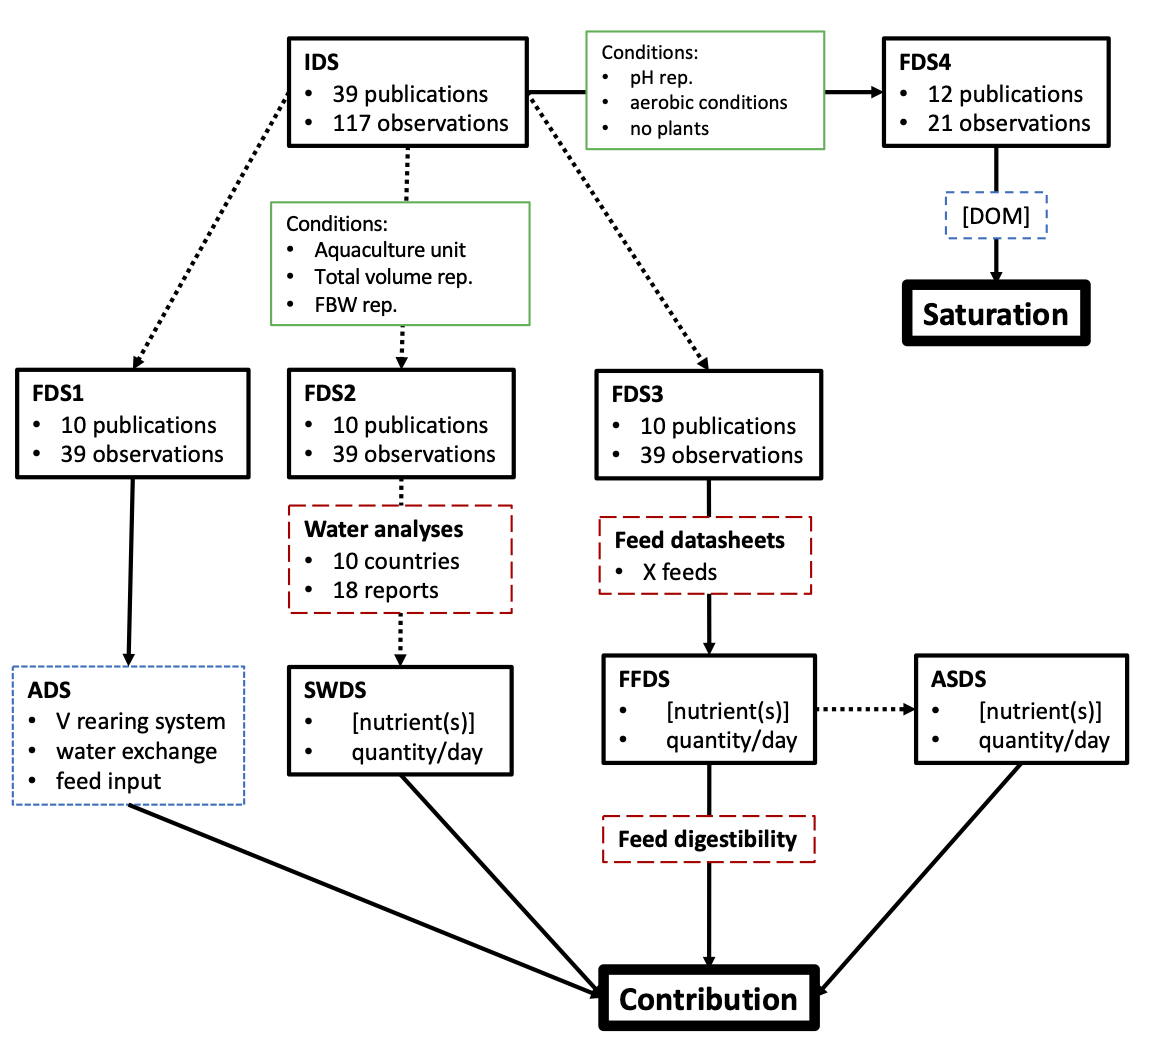
\includegraphics{images/data_analysis_flow.png}
\caption{Graphical representation of the data acquition and wrangling steps. IDS: Initial dataset; FDS1 and 2: Filtered datasets; SWDS: Source water dataset; FIDS: Feed information dataset; ASDS: Alkalinity supplements dataset;
Green box: filter applied; red box: external data added; solid line: dataset; dotted line: data derived from initial dataset; dashed line: data derived from external source; thick solid line: final usage of data.}
\end{figure}

\hypertarget{origin-of-nutrients}{%
\subsection{Origin of nutrients}\label{origin-of-nutrients}}

To calculate the proportion contribution of the source water, feed and alkalinity supplements to the total daily nutrient input in the reviewed studies, their average daily inputs per volume unit had to be calculated. For this purpose, statistics describing the average experimental system, system parameters and nutrient inputs were derived from the IDS and merged with external data sources in a four-stage process.
The first step comprised the generation of system assumptions. For this purpose, a filter was applied to the IDS, only including studies that made use of an aquaculture unit, reported the total system volume and the final bodyweight of the livestock at the end of the experiment. The resulting filtered dataset (FDS1) held 39 observations from 10 publications.

\begin{Shaded}
\begin{Highlighting}[]
\FunctionTok{read\_csv}\NormalTok{(}\FunctionTok{here}\NormalTok{(}\StringTok{"results"}\NormalTok{, }\StringTok{"contribution\_rearing\_data.csv"}\NormalTok{)) }\SpecialCharTok{\%\textgreater{}\%} 
  \FunctionTok{summarise}\NormalTok{(}
    \AttributeTok{observations =} \FunctionTok{n}\NormalTok{(),}
    \AttributeTok{publications =} \FunctionTok{length}\NormalTok{(}\FunctionTok{unique}\NormalTok{(Reference\_ID))}
\NormalTok{  )}
\end{Highlighting}
\end{Shaded}

\begin{verbatim}
## Rows: 39 Columns: 30
## -- Column specification --------------------------------------------------------
## Delimiter: ","
## chr  (7): Reference_ID, species, Treatment_ID, site, city, country, Survival
## dbl (23): IBW_g, days, tankV_m3, tankN, Vmisc_m3, totalV_m3, density_kg_m3, ...
## 
## i Use `spec()` to retrieve the full column specification for this data.
## i Specify the column types or set `show_col_types = FALSE` to quiet this message.
\end{verbatim}

\begin{verbatim}
## # A tibble: 1 x 2
##   observations publications
##          <int>        <int>
## 1           39           10
\end{verbatim}

\begin{Shaded}
\begin{Highlighting}[]
\FunctionTok{read\_csv}\NormalTok{(}\FunctionTok{here}\NormalTok{(}\StringTok{"results"}\NormalTok{, }\StringTok{"contribution\_rearing\_data.csv"}\NormalTok{)) }\SpecialCharTok{\%\textgreater{}\%} 
  \FunctionTok{summarise}\NormalTok{(}
    \FunctionTok{unique}\NormalTok{(Reference\_ID)}
\NormalTok{  )}
\end{Highlighting}
\end{Shaded}

\begin{verbatim}
## Rows: 39 Columns: 30
## -- Column specification --------------------------------------------------------
## Delimiter: ","
## chr  (7): Reference_ID, species, Treatment_ID, site, city, country, Survival
## dbl (23): IBW_g, days, tankV_m3, tankN, Vmisc_m3, totalV_m3, density_kg_m3, ...
## 
## i Use `spec()` to retrieve the full column specification for this data.
## i Specify the column types or set `show_col_types = FALSE` to quiet this message.
\end{verbatim}

\begin{verbatim}
## # A tibble: 10 x 1
##    `unique(Reference_ID)`
##    <chr>                 
##  1 Shaw2022a             
##  2 Monsees2017b          
##  3 Siqwepu2020           
##  4 Knaus2022             
##  5 Schmautz2016          
##  6 Knaus2020             
##  7 Pasch2021             
##  8 Pasch2021a            
##  9 Delaide2017           
## 10 Knaus2017
\end{verbatim}

FDS1 was used to calculate the average system volume (\(\text{V}_{tot}\)), average bodyweight (\(ABW\)), average number of livestock (\(AN\)), average livestock density (\(AD\)), and average water exchange rate (\(AWE\)). \(ABW\) was defined as the mean bodyweight during the duration of experiment and was calculated as the arithmetic mean of the initial and final bodyweight. For the calculation of \(AD\), \(AN\) and \(AWE\), \emph{NA} values were removed.
Eventually, the average biomass (\(ABM\)) was computed by multiplication of \(ABW\) with \(AN\) or, if only \(AD\) was given, by multiplication of \(AD\) with \(\text{V}_{tot}\). Vice versa, in case \(AD\) was not reported, it was calculated by dividing \(ABM\) by \(\text{V}_{tot}\). The average daily water exchange volume by multiplication of (\(\text{V}_{tot}\)) with \(AWE\).

The second step was the estimation of the daily nutrient input via source water. For this purpose, gathered location information in the FDS was used to search for water analysis reports provided by the closest water treatment plant. Only official reports provided by local authorities and water utilities in the corresponding municipalities were used to ensure that analyses were conducted according to internationally accepted laboratory standards.
In water analysis, it is common practice to report the value of the detection limit instead of the measured value in case that the analyte concentration found was below the sensitivity of the instrument used for measurement (Deutsches Institut für Normung e.V. 2008). Retaining the detection limits in the dataset leads to mean concentration estimates that are too large. However, removing the affected observations would result in a loss a large proportion of the data, as shown in \textbf{FIGURE XXX}. Therefore, concentration data was recalculated using the \emph{cenmle()} function from the R package \emph{NADA} by maximum likelihood estimation (MLE) (\textbf{Helsel2012?}). This ensured that the estimates for nutrient concentrations in tap water were reliable.

\begin{figure}
\centering
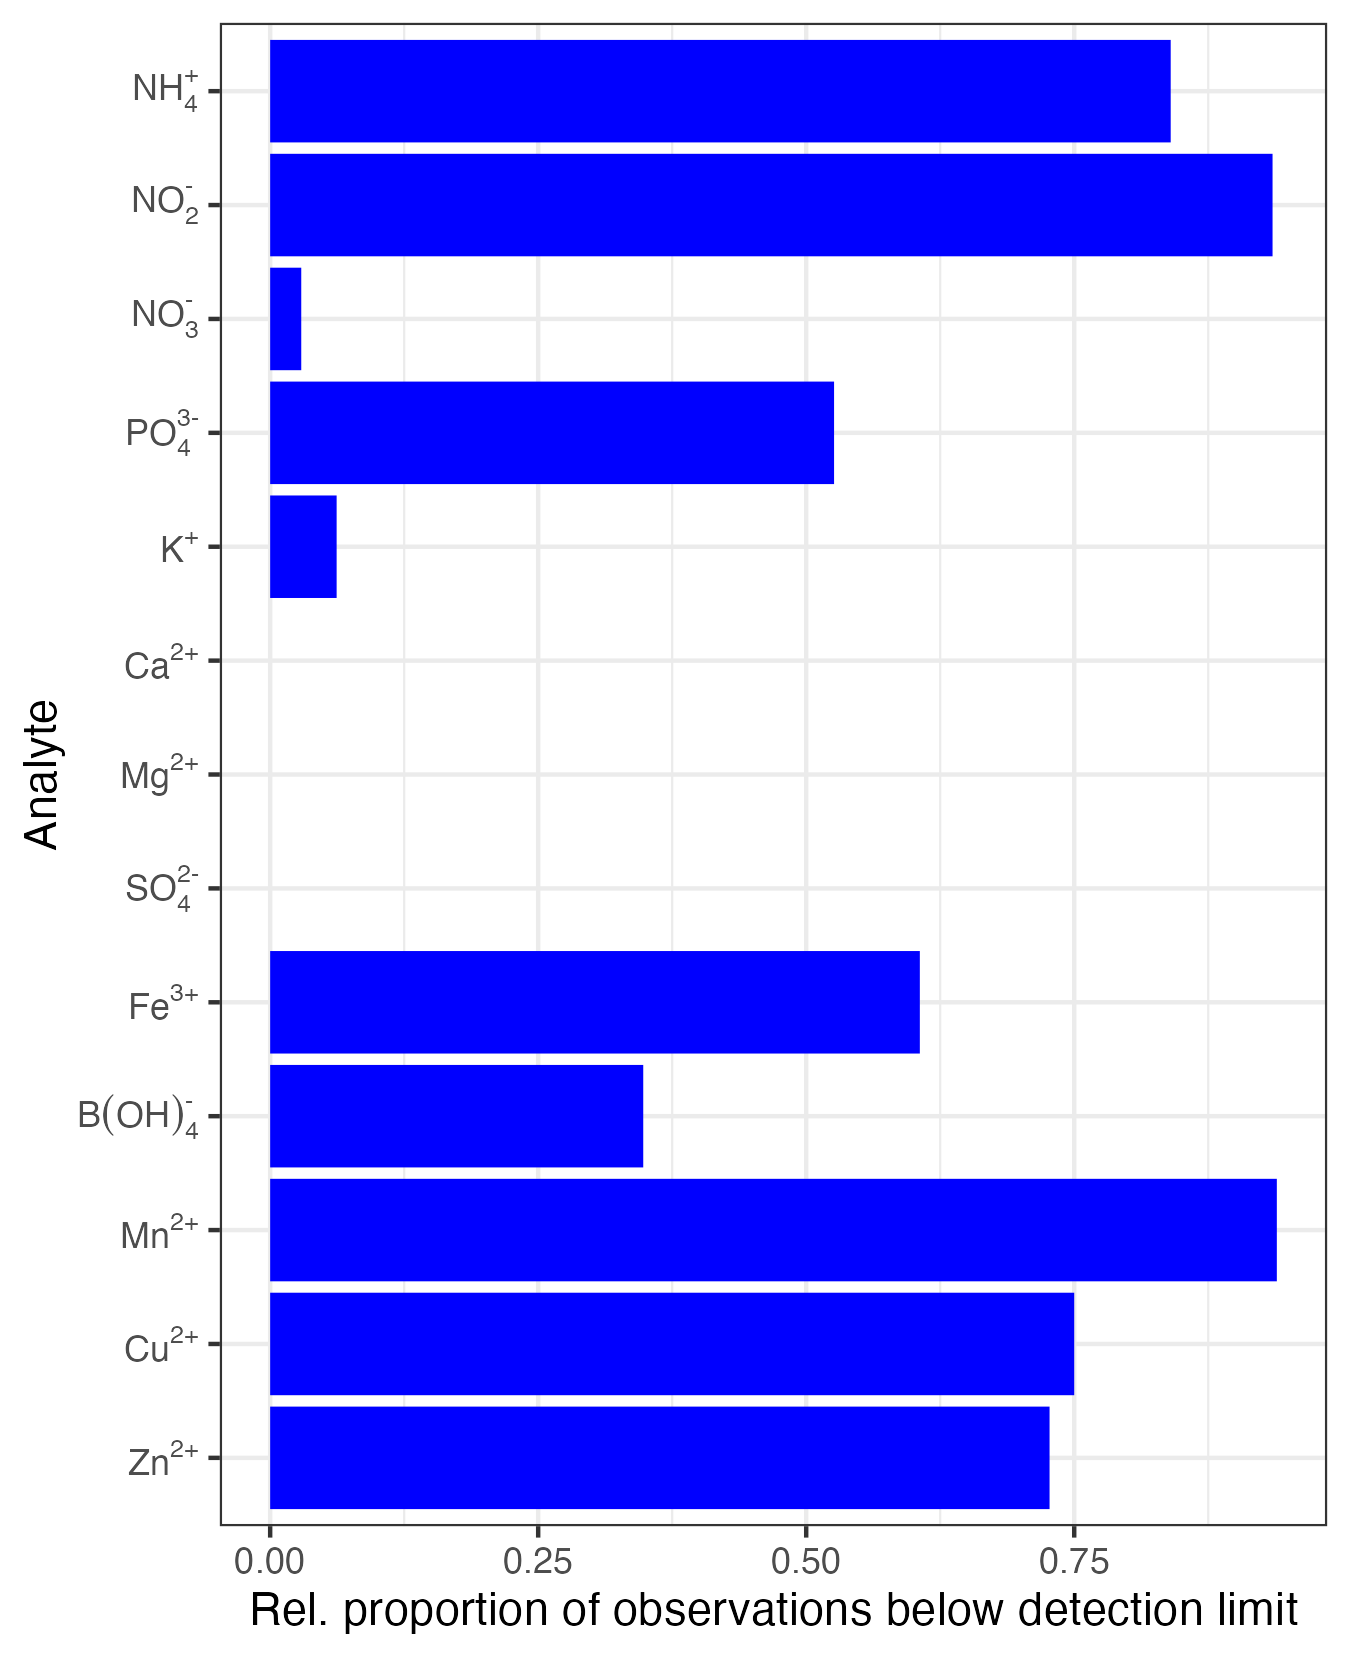
\includegraphics{plots/contribution_waterData_belowLimit.png}
\caption{Proportion of water analysis observations per analyte reported to be below detection limit (n = XXX).}
\end{figure}

The output was eventually used to calculate the two-sided 90\% confidence interval for the concentration of each nutrient to describe the concentration range that will be found in 90\% of all cases where tap water is used.
Finally, multiplying the obtained concentrations with \(AWE\) yielded the upper and lower limits of the 90\% confidence interval of total daily individual plant nutrient inputs via source water.

In the third step, daily nutrient inputs via aquafeeds were estimated. The IDS was filtered for studies reporting the name of the commercial aquafeed used (if not selfmade), the \(CP\) inclusion rate and the feeding rate. From the resulting FDS2, the average feeding rate (\(AFR\)), \(CP\) inclusion rate (\(ACP\)) and the averages of all plant nutrients were calculated. Due to lacking nutrient composition data, supplier datasheets were used and amended by literature data in case of utilization of commercial aquafeeds. Incomplete observations with respect to experimental feeds were handled in the same way, merging data from multiple publications if the same feed was used. \emph{NA} values were removed for the computation of averages.
Eventually, the average daily feed input (\(AFI\)) was calculated by multiplying ABM from the generated system assumptions with AFR. By multiplying \(AFI\) with the average plant nutrient inclusion rates in the aquafeeds, the uncorrected total daily input of individual plant nutrients via aquafeeds could be calculated. Obtained values were then corrected by multiplication with apparent digestibility coefficients (\(ADC\)), accounting for the digestibility of aquafeeds by fish. An \(ADC\) of 90\% was assumed for N whereas the \(ADC\) of all other nutrients was assumed to be 50\% (Lall Fish Nutrition The Minerals, 2002). Finally, it was assumed that 50\% of the digestible fraction is retained while the remaining 50\% is excreted in dissolved form (\textbf{Halver2003?}). The indigestible part of the feed is excreted as solid feces and was thus assumed not to participate in chemical reactions in solution.

An estimate for the daily input of alkalinity supplements was derived from \(AFI\). The activity of nitrifying bacteria in the biofilter follows the overall simplified reaction

\[
\text{NH}_{4}^{+} + 2 \text{ O}_{2} \rightarrow \text{NO}_{3}^{-} + 2 \text{ H}^{+} + \text{ H}_{2}\text{O}
\]

(Timmons 2010), thus releasing two moles of protons (H\(^{+}\)) per mole of ammonium (\(\text{NH}_{4}^{+}\)) that is converted to nitrate (\(\text{NO}_{3}^{-}\)). Neutralization of these protons has to take place to counteract the resulting decrease in pH. Thus, the amounts of \(\text{NaHCO}_{3}\), \(\text{KOH}\) or \(\text{Ca(OH)}_{2}\) that are necessary to neutralise the released protons were calculated by assuming that the digestible, non-retained proportion of \(CP\) is excreted as \(\text{NH}_{4}^{+}\).

\[
AFI \frac{CP}{f_{K}} \cdot \frac{f_{S}\text{M(H)}}{\text{M(N)}}
\]

with \(f_{K} = 6.25\), denoting for the Kjeldahl factor.

\[
\text{NH}_{4}^{+} + 1.83 \text{ O}_{2} + 1.97 \text{ HCO}_{3} \rightarrow 0.0244 \text{C}_{5}\text{H}_{7}\text{O}_{2}\text{N} + 0.976 \text{ NO}_{3}^{-} + 2.90 \text{ H}_{2}\text{O} + 1.86 \text{ CO}_{2}
\]
(Timmons 2010), thus consuming \(1.97 \text{ mol} \cdot 60.71 \text{g mol}^{-1} = 119.5 \text{g}\) of

releasing two moles of protons (H\(^{+}\)) per mole of ammonium (\(\text{NH}_{4}^{+}\)) that is converted to nitrate (\(\text{NO}_{3}^{-}\)). To counteract the resulting decrease in pH

This leads to a decrease in pH over time and consequently to a decrease in the activity of the nitrifyers (Ward, Arp, and Klotz 2011). NH\(_{3}\) results from the metabolization of CP

\hypertarget{fate-and-behavior-of-nutrients}{%
\subsection{Fate and behavior of nutrients}\label{fate-and-behavior-of-nutrients}}

\hypertarget{assumptions-and-data-selection}{%
\subsubsection{Assumptions and data selection}\label{assumptions-and-data-selection}}

Due to aeration of the RAS tanks and the oxygen requirements of the livestock and nitrifyers, it was assumed that aerobic conditions are predominant in all systems. This would lead to the presence of metals in their reduced forms, e.g.~{[}Fe\(^{3+}\){]} \textgreater\textgreater{} {[}Fe\(^{2+}\){]}. Furthermore, it was assumed that CO\(_{2}\) in solution is in equilibrium with CO\(_{2}\) in the atmosphere. According to Henry's Law, this would result in a concentration of {[}CO\(_{2}\)(aq){]}\(_{total} = K_{H} \cdot p_{\text{CO}_{2}} = 0.018\) mol L\(^{-1}\), assuming a partial pressure \(p_{\text{CO}_{2}} = 0.054\) atm and the corresponding Henry constant of \(K_{H} = 3.4 \cdot 10^{-2}\) mol L\(^{-1}\) atm\(^{-1}\) (Stumm 1981).

Data from the aquaponics dataset was used and observations originating from aquaponic studies were limited to those making use of an on-demand coupled system design to ensure that measured analyte concentrations were not impacted by plant uptake. Furthermore, anaerobic treatments were excluded from data originating from sludge remineralisation studies. The number of observations in the initial dataset was further reduced by excluding those that did not report pH, leading to a final dataset of 25 observations originating from 16 publications.

\hypertarget{complexation-by-dissolved-organic-matter}{%
\subsubsection{Complexation by dissolved organic matter}\label{complexation-by-dissolved-organic-matter}}

The complexation of plant nutrients by dissolved organic matter (DOM) was simulated using the Gaussian DOM model (Grimm et al. 1991). It was assumed that DOM is present in the systems at a concentration of 20 mg L\(^{-1}\). The charge of the DOM species was calculated according to database values.

\hypertarget{mineral-saturation-and-precipitation}{%
\subsubsection{Mineral saturation and precipitation}\label{mineral-saturation-and-precipitation}}

To assess whether the waters in the selected literature were saturated with regards to specific minerals, mineral saturation indices \(\log(\frac{Q}{K})\) were calculated. The saturation index of a mineral is the ratio between its ion product \(Q\) and its solubility product \(K_{sp}\). \(Q\) can be generally expressed as follows

\[
Q = [\text{cation}(aq)]^n \cdot [\text{anion}(aq)]^m
\]

where the expressions in square brackets denote for the empirically found concentrations of the cationic and anionic components of a mineral taken to the power of their stoichiometric coefficients \(m\) and \(n\). For instance, a concentration of {[}Fe\(^{3+}\){]} = {[}PO\(_{4}^{3-}\){]} = 0.1 mol \(\text{L}^{-1}\) would result in \(Q = [\text{Fe}^{3+}]^1 \cdot [\text{PO}_{4}^{3-}]^1 = 0.01 \text{ mol}^2 \text{ L}^2\). \(K_{sp}\) is calculated analogously to the ion product but with concentrations denoting for the saturation concentration that is reached when a solid mineral equilibrates with its dissolved ions. If \(\log(\frac{Q}{K}) = 0\), the concentration of ions is higher than their solubility under equilibrium conditions. The solution is thus not thermodynamically stable and the correpsonding mineral is precipitating. On the other hand, if \(\log(\frac{Q}{K}) < 0\), more of the solid mineral can dissolve until the equilibrium concentration is reached. In case that \(\log(\frac{Q}{K}) > 0\), there are other factors such as complexation reactions that are increasing the solubility.

All observations that were affected by precipitation (\(\log(\frac{Q}{K}) = 0\)) were eventually tested with regards to the concentration proportion that precipitated of the affected nutrient.

\hypertarget{results}{%
\section{Results}\label{results}}

\hypertarget{gathered-data-and-derived-assumptions}{%
\subsection{Gathered data and derived assumptions}\label{gathered-data-and-derived-assumptions}}

\hypertarget{rearing-data}{%
\subsubsection{Rearing data}\label{rearing-data}}

Assumptions were derived from studies about aquaponic systems to calculate contributions of nutrient sources to daily nutrient inputs into the system.
Analysis of the data presented in the reviewed aquaponics studies revealed that the average total water volume of the aquaculture systems was 4.53 m\(^{3}\) with an average volume of the rearing compartment of 2.81 m\(^3\). An average stocking density, calculated as the average of the initial and final density, of 7.69 kg m\(^{-3}\), feeding rate of 2\%, and water exchange rate of 3\% were found.

As shown in \textbf{FIGURE XXX}, literature data comprised a total of nine different cultivated fish species, of which four were cyprinids, three percids, one silurid and salmonid species, respectively. Percid fish were cultivated in 63\% and Silurids in 23\% of the studies, while Cyprinids were used in 10\% and Salmonids in only 2\% of the studies.

\begin{figure}
\centering
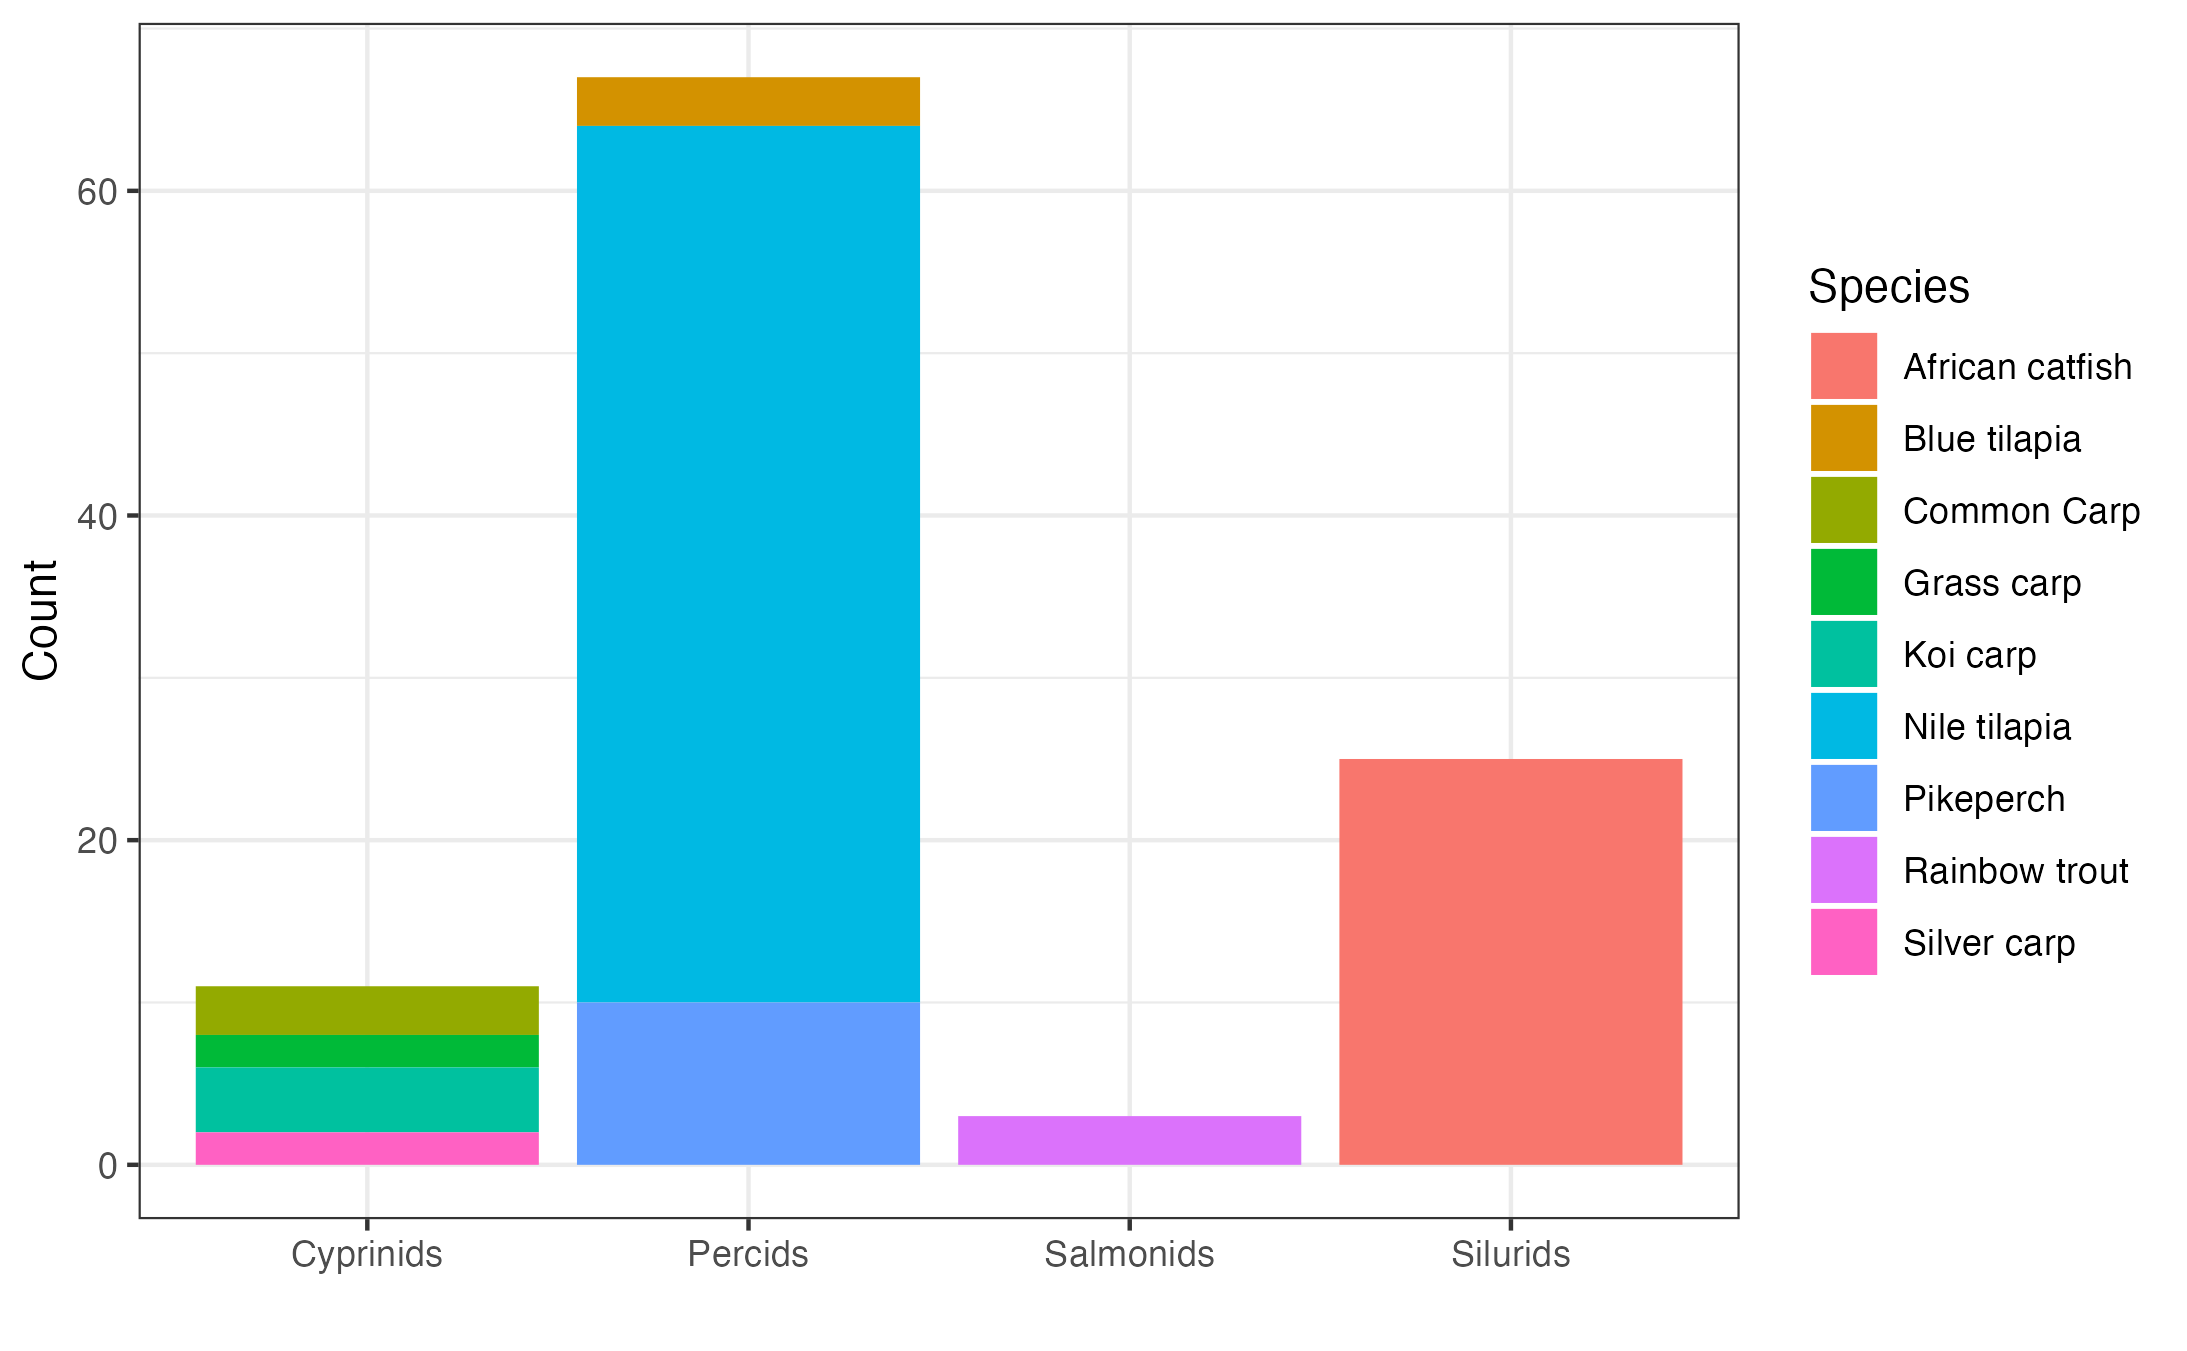
\includegraphics{plots/species.png}
\caption{Overview of species reared during aquaponic experiments}
\end{figure}

\hypertarget{water-data}{%
\subsubsection{Water data}\label{water-data}}

\begin{Shaded}
\begin{Highlighting}[]
\FunctionTok{read\_csv}\NormalTok{(here}\SpecialCharTok{::}\FunctionTok{here}\NormalTok{(}\StringTok{"results"}\NormalTok{, }\StringTok{"contribution\_water\_countries.csv"}\NormalTok{)) }\SpecialCharTok{\%\textgreater{}\%} 
  \FunctionTok{group\_by}\NormalTok{(Source, Country) }\SpecialCharTok{\%\textgreater{}\%} 
  \FunctionTok{summarise}\NormalTok{(}\AttributeTok{n =} \FunctionTok{n}\NormalTok{()) }\SpecialCharTok{\%\textgreater{}\%} 
  \FunctionTok{group\_by}\NormalTok{(Source) }\SpecialCharTok{\%\textgreater{}\%} 
  \FunctionTok{summarise}\NormalTok{(}\AttributeTok{n =} \FunctionTok{n}\NormalTok{())}
\end{Highlighting}
\end{Shaded}

\begin{verbatim}
## Rows: 76 Columns: 48
## -- Column specification --------------------------------------------------------
## Delimiter: ","
## chr  (6): City, Country, Source, Reference_ID, Location, Aquaponics
## dbl (22): Year, pH, EC_uS_cm_25degC, NH4_mgL, NO2_mgL, NO3_mgL, PO4_mgL, K_m...
## lgl (20): ZIP, NH4_belowLimit, NO2_belowLimit, NO3_belowLimit, PO4_belowLimi...
## 
## i Use `spec()` to retrieve the full column specification for this data.
## i Specify the column types or set `show_col_types = FALSE` to quiet this message.
## `summarise()` has grouped output by 'Source'. You can override using the `.groups` argument.
\end{verbatim}

\begin{verbatim}
## # A tibble: 2 x 2
##   Source         n
##   <chr>      <int>
## 1 Literature    12
## 2 Reports       12
\end{verbatim}

Literature data consisted of studies from a total of twelve countries. The country distribution of the literature data in comparison with obtained water analysis reports is shown in \textbf{FIGURE XXX}.

\begin{figure}
\centering
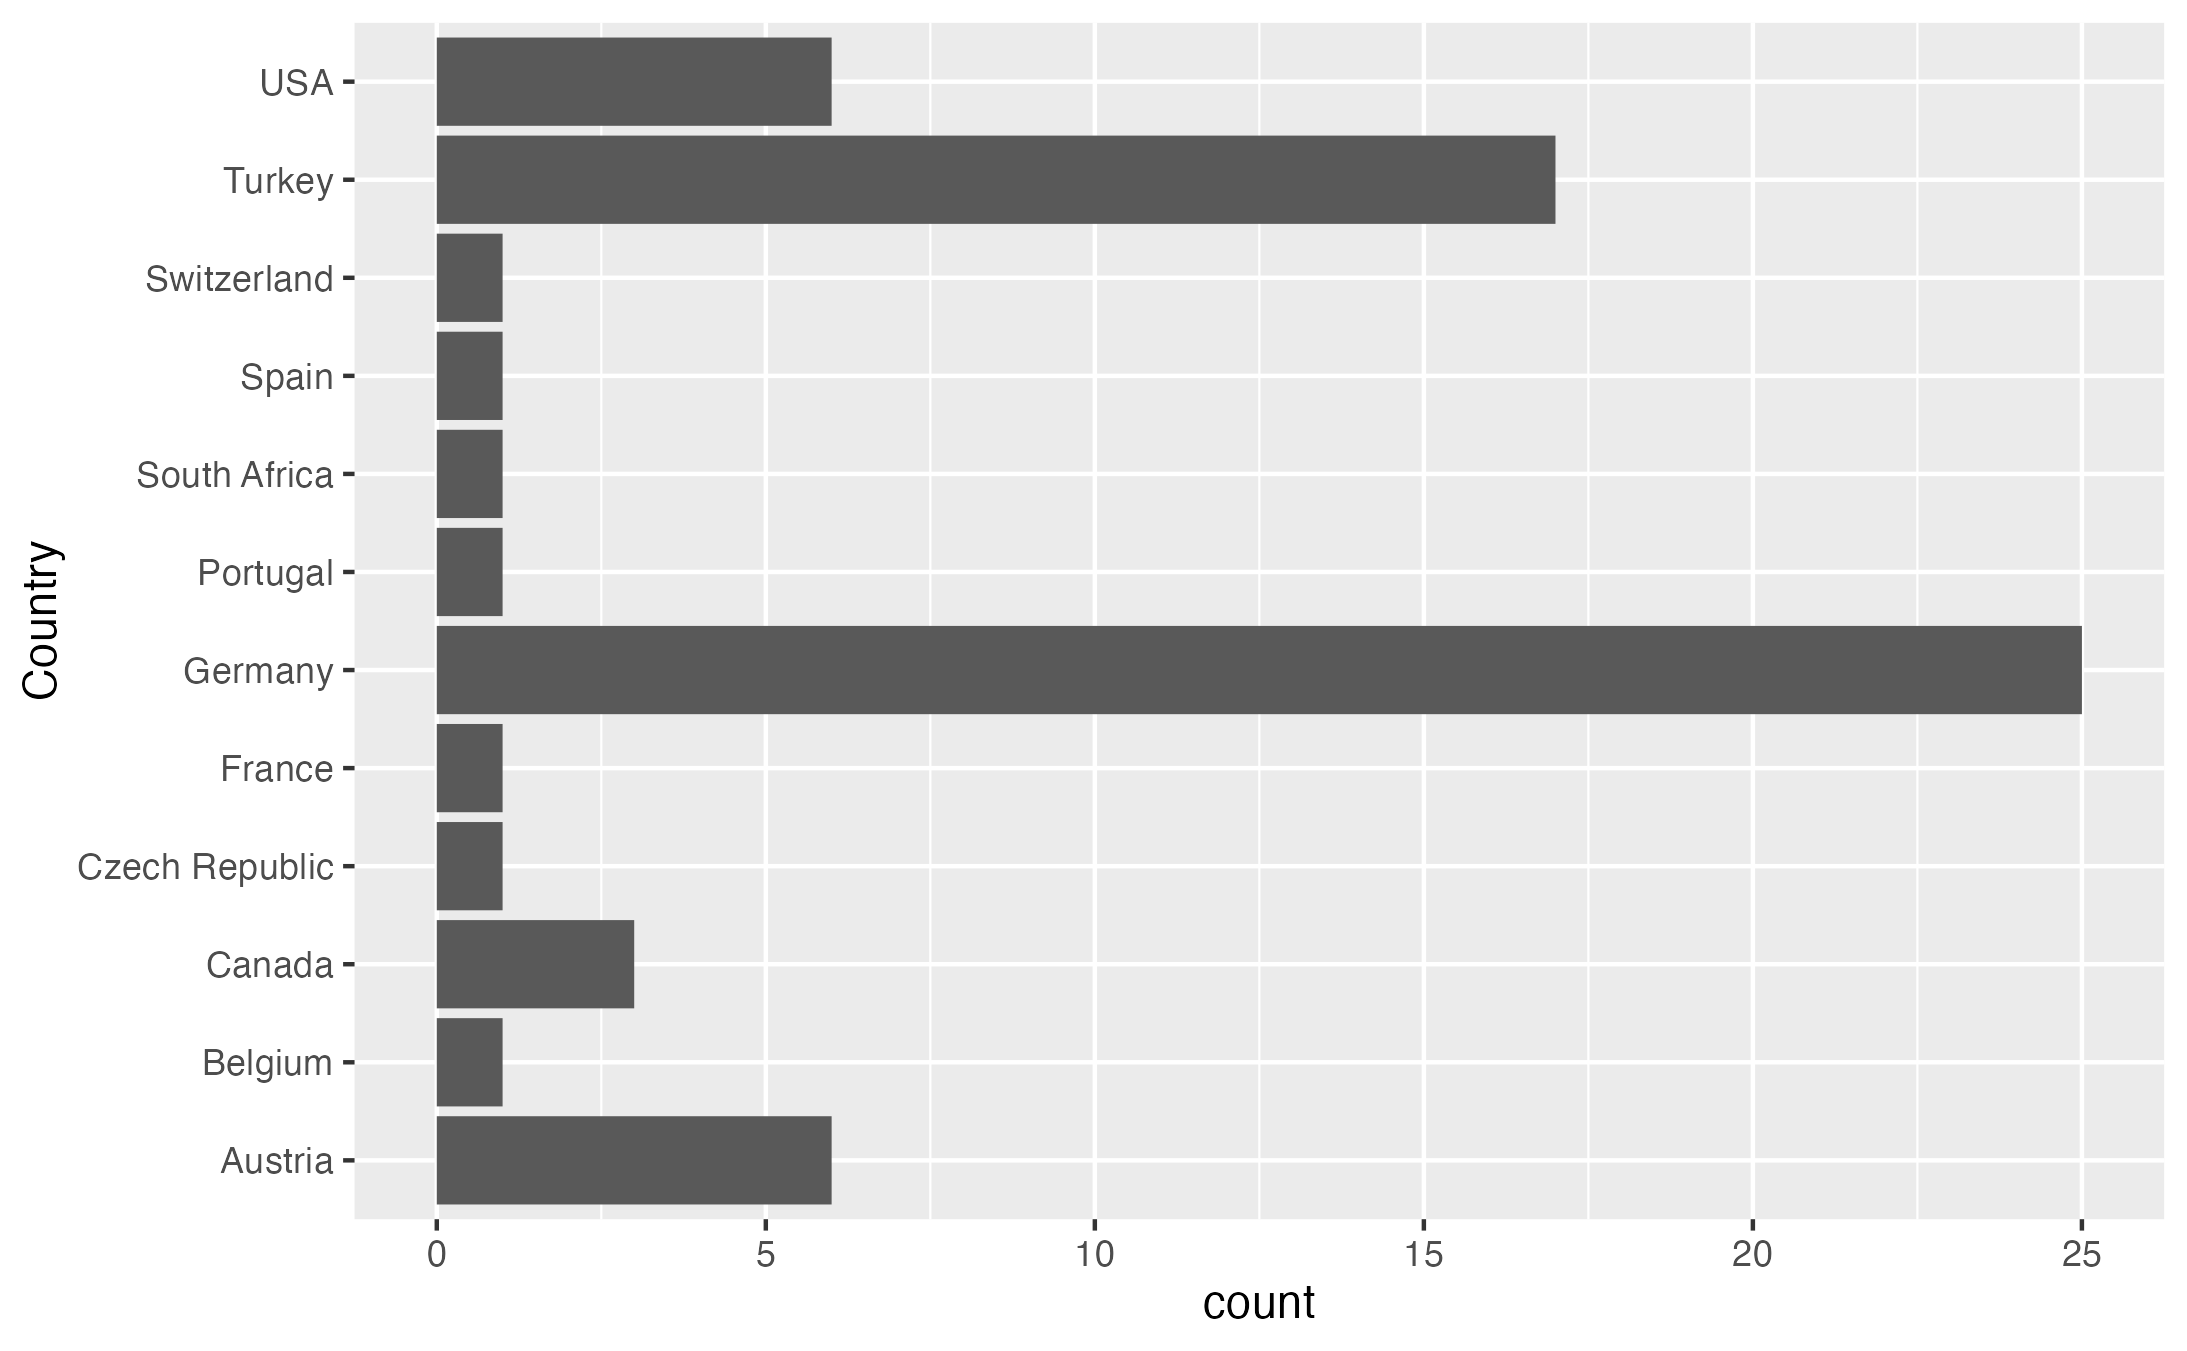
\includegraphics{plots/contribution_waterData_countryPlot.png}
\caption{Number of studies per country in comparison with the number of water analysis reports per country included in the source water dataset.}
\end{figure}

\hypertarget{nutrient-sources}{%
\subsection{Nutrient sources}\label{nutrient-sources}}

Using the assumptions derived from literature, an average biomass of 40.98 kg and daily inputs of \(40.98 \text{ kg} \cdot 2\% = 0.8\) kg of feed with an average crude protein content of 41\% on dry matter basis and \(4.53 \text{ m}^{3} \cdot 3\% = 0.14 \text{ m}^{3}\) of freshwater were calculated.

The daily feed input and crude protein content resulted in a daily N input of \(\frac{0.8 \text{ kg d}^{-1} \cdot 41\%}{6.25} \cdot 1000 \frac{\text{g}}{\text{mg}} = 52.4 \text{ g d}^{-1}\).
Nitrification, under the assumption that This generated H\(^{+}\) required \(\frac{52.4 \text{ g}}{14 \text{ g mol}^{-1}} = 3.7\) mol d\(^{-1}\) of H\(^{+}\) to be neutralized. For this purpose, the input of the same amount of \(\text{NaHCO}_{3}\), KOH or half of Ca(OH)\(_{2}\) would be required, resulting in an input of 190.5 g d\(^{-1}\) K or 97.6 g d\(^{-1}\) of Ca.

The average nutrient composition of both aquafeeds and source water and the lower and upper limits of the 95\% confidence interval for source water are shown in \textbf{TABLE XXX}.
It is evident that the highest daily nutrient input usually originates from the aquafeeds

\textbf{Compositions of nutrient sources and daily inputs. Shown are the averages for both aquafeeds and source water and the lower and upper limits of the 95\% confidence interval for the source water.}
Source water: n = 64;Aquafeeds: n = 54

\begin{longtable}[]{@{}
  >{\raggedright\arraybackslash}p{(\columnwidth - 12\tabcolsep) * \real{0.1429}}
  >{\raggedright\arraybackslash}p{(\columnwidth - 12\tabcolsep) * \real{0.1429}}
  >{\raggedright\arraybackslash}p{(\columnwidth - 12\tabcolsep) * \real{0.1429}}
  >{\raggedright\arraybackslash}p{(\columnwidth - 12\tabcolsep) * \real{0.1429}}
  >{\raggedright\arraybackslash}p{(\columnwidth - 12\tabcolsep) * \real{0.1429}}
  >{\raggedright\arraybackslash}p{(\columnwidth - 12\tabcolsep) * \real{0.1429}}
  >{\raggedright\arraybackslash}p{(\columnwidth - 12\tabcolsep) * \real{0.1429}}@{}}
\toprule()
\begin{minipage}[b]{\linewidth}\raggedright
Nutrient
\end{minipage} & \begin{minipage}[b]{\linewidth}\raggedright
Aquafeeds
\end{minipage} & \begin{minipage}[b]{\linewidth}\raggedright
Source water
\end{minipage} & \begin{minipage}[b]{\linewidth}\raggedright
pH management
\end{minipage} & \begin{minipage}[b]{\linewidth}\raggedright
Aquafeeds daily
\end{minipage} & \begin{minipage}[b]{\linewidth}\raggedright
Source water daily
\end{minipage} & \begin{minipage}[b]{\linewidth}\raggedright
pH management daily
\end{minipage} \\
\midrule()
\endhead
N & 66.3 g kg\(^{-1}\) & 1.2 mg L\(^{-1}\) {[}0.8, 1.7{]} & - & & 5.680 g d\(^{-1}\) & - \\
P & 8.8 g kg\(^{-1}\) & 95.2 µg L\(^{-1}\) {[}34.4, 156.0{]} & - & & 0.419 g d\(^{-1}\) & - \\
K & 7.1 g kg\(^{-1}\) & 2.6 mg L\(^{-1}\) {[}1.8, 3.4{]} & & & 11.685 g d\(^{-1}\) & 487.0 g d\(^{-1}\) \\
Ca & 15.9 g kg\(^{-1}\) & 64.4 mg L\(^{-1}\) {[}55.6, 73.2{]} & & & 283.477 g d\(^{-1}\) & 249.6 g d\(^{-1}\) \\
Mg & 2.0 g kg\(^{-1}\) & 11.5 mg L\(^{-1}\) {[}9.4, 13.6{]} & - & & 50.644 g d\(^{-1}\) & - \\
S & 3.9 g kg\(^{-1}\) & 14.2 mg L\(^{-1}\) {[}10.7, 17.8{]} & - & & 62.763 g d\(^{-1}\) & - \\
B & 17.1 mg kg\(^{-1}\) & 48.9 µg L\(^{-1}\) {[}34.6, 63.3{]} & - & & 215.5 mg d\(^{-1}\) & - \\
Fe & 291.3 mg kg\(^{-1}\) & 18.7 µg L\(^{-1}\) {[}12.3, 25.1{]} & - & & 82.5 mg d\(^{-1}\) & - \\
Mn & 71.9 mg kg\(^{-1}\) & 5.8 µg L\(^{-1}\) {[}2.9, 8.7{]} & - & & 25.6 mg d\(^{-1}\) & - \\
Cu & 14.3 mg kg\(^{-1}\) & 22.4 µg L\(^{-1}\) {[}0, 45.7{]} & - & & 98.7 mg d\(^{-1}\) & - \\
Zn & 169.7 mg kg\(^{-1}\) & 13.9 µg L\(^{-1}\) {[}0, 28.2{]} & - & & 61.5 mg d\(^{-1}\) & - \\
Mo & 1.7 mg kg\(^{-1}\) & 0.7 µg L\(^{-1}\) {[}0.5, 1.0{]} & - & & 0.3 mg d\(^{-1}\) & - \\
Ni & 0.9 mg kg\(^{-1}\) & 1.6 µg L\(^{-1}\) {[}1.0, 2.2{]} & - & & 7.4 mg d\(^{-1}\) & - \\
Na & & 25.5 mg d\(^{-1}\) & - & & 112.343 g d\(^{-1}\) & 286.3 g d\(^{-1}\) \\
\bottomrule()
\end{longtable}

\textbf{Figure XXX} visualises the proportion of the daily total nutrient inputs from each nutrient source after consideration of aquafeed digestibility.
The results confirm that aquafeeds were the main nutrient source in the reviewed studies. Considering the range of the possible nutrient contribution by source water that is given by the upper and lower limits of the 95\% confidence interval, it was found that aquafeeds provided between 99.8\% and 99.9\% of N, 99.7\% and 99.9\% of P, 94.4\% and 94.4\% and 96.8\% of K. They were thus contributing almost nearly the total amount of the most important macronutrients. In addition, aquafeeds were the main contributors to the daily total input of Fe (98.9\% to 99.4\%), Mn (98.5\% to 99.5\%), Mo (93.0\% to 96.4\%), and Zn (98.0\% to 100\%). The variability for these plant nutrients was comparably low.
The most variable plant nutrient with respect to its source concentration was found to be Cu with a contribution of aquafeeds between 71.9\% and 100\% to the total daily inputs. The variability of the following plant nutrients decreased in descending order: B (68.8\% to 80.1\%), Ni (75.5\% to 86.6\%), S (64.1\% to 74.8\%), Mg (54.0\% to 62.9\%), and Ca (64.1\% to 70.1\%).
Interestingly, aquafeeds were found not to be the predominant input route of Na (38.4\% to 55.7\%) on average.
show the same plots under addition of KOH and Ca(OH)\(_{2}\) to adjust the pH, respectively.
It becomes evident that the addition of pH adjusting substances results in them becoming the main input route of the cation they are containing (K, Ca or Na).
decreasing the share of the feed from XXX\% to YYY\% if KOH is added. The use of Ca(OH)\(_{2}\) leads to only half of the molar input of Ca compared to K as its hydroxide contains two hydroxide ions. However, it is still contributing almost 100\% of the daily total Ca input while the shares of feed and water are dropping to XXX\% and YYY\%, respectively.

\begin{figure}
\centering
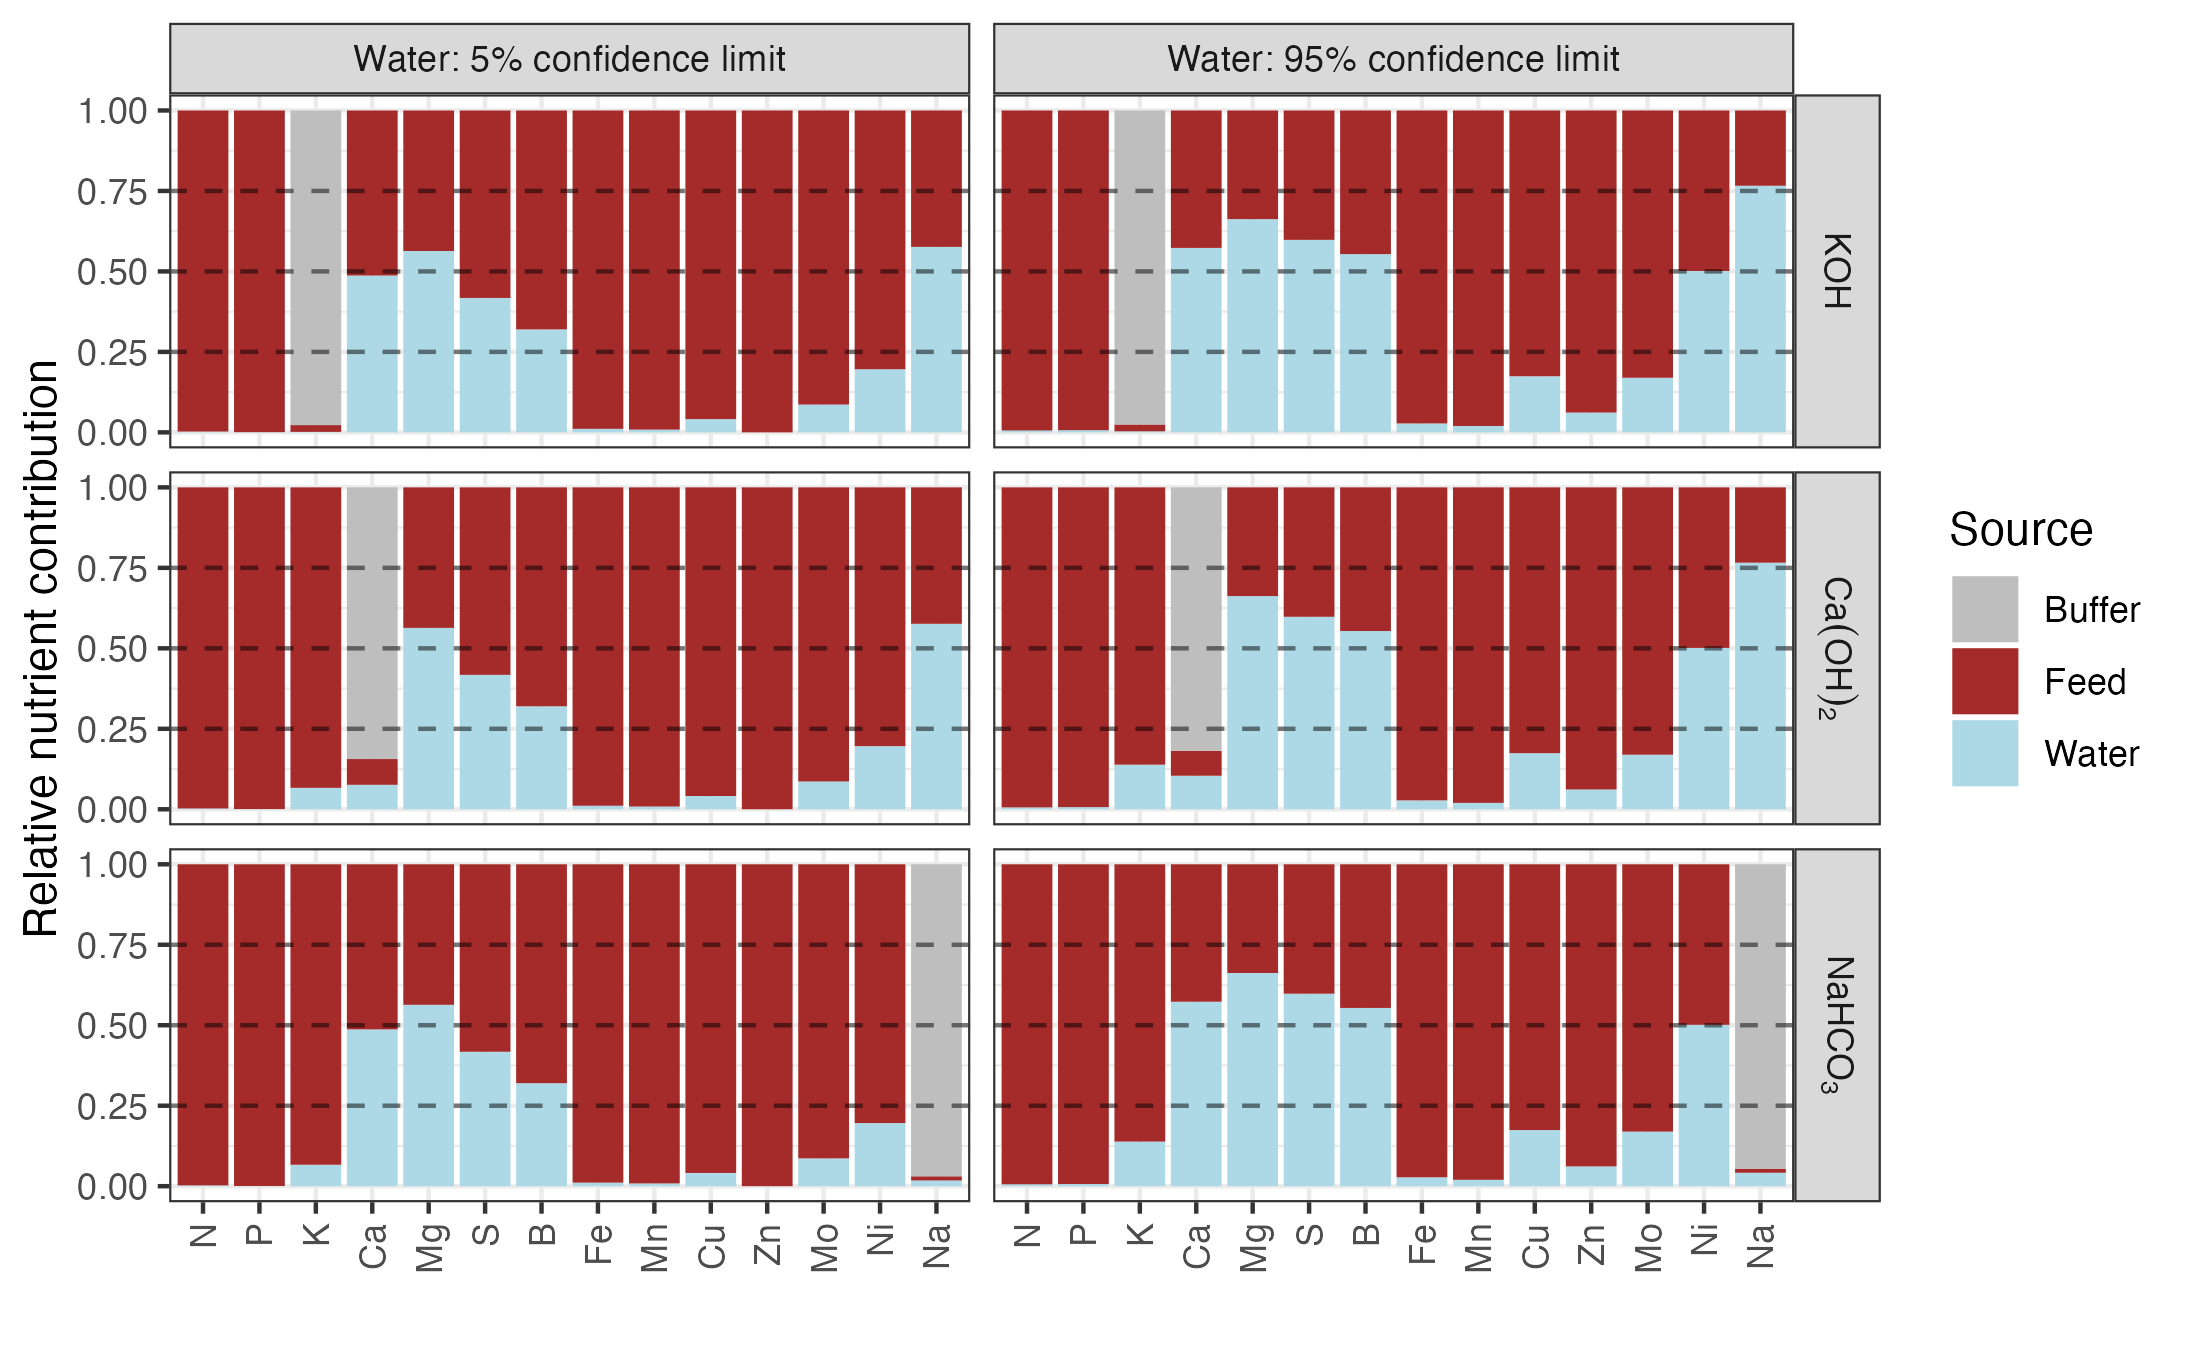
\includegraphics{plots/contribution_sources_digestincl.png}
\caption{Relative contribution of source water, feed and substances for pH management to the total daily nutrient input in aquaculture and aquaponic systems. Shown are scenarios reflecting the lower and upper limit of the 95\% confidence interval of concentration data for source water. Data derived from water analysis (n = 69) and feed analysis reports (n = 9), taking digestibility into account, assuming 90\% apparent digestibility of N, 50\% apparent digestibility of all other plant nutrients, 100\% purity and no contribution of pH management substances to other nutrient inputs.}
\end{figure}

\hypertarget{fate-and-behavior-of-nutrients-1}{%
\subsection{Fate and behavior of nutrients}\label{fate-and-behavior-of-nutrients-1}}

The proportion of potential cation complexation by DOM was calculated to assess the possible impact of DOM on the solubility of plant nutrients in the reviewed studies. The results are shown in \textbf{FIGURE XXX}.

Under the given assumption of a DOM concentration of \(20 \text{ mg L}^{-1}\) and the use of a Gaussian DOM model, five cationic nutrients, namely Ca, Mg, Fe, Cu and Zn, were found to be possibly affected by DOM.
The highest average affinity for the formation of complex molecules was found for Cu with a complexed proportion of \(42.6\% \pm 33\%\) of the total concentration in solution, followed by Ca (\(21.2\% \pm 18\%\)) and Zn (\(11.9\% \pm 14\%\)). These three compounds also showed the highest variability with respect to their interactions with DOM. Based on the model predictions, less interaction with DOM was found between Mg (\(3.0\% \pm 6\%\)) and Fe (\(0.1\% \pm 0.1\%\)).

\begin{figure}
\centering
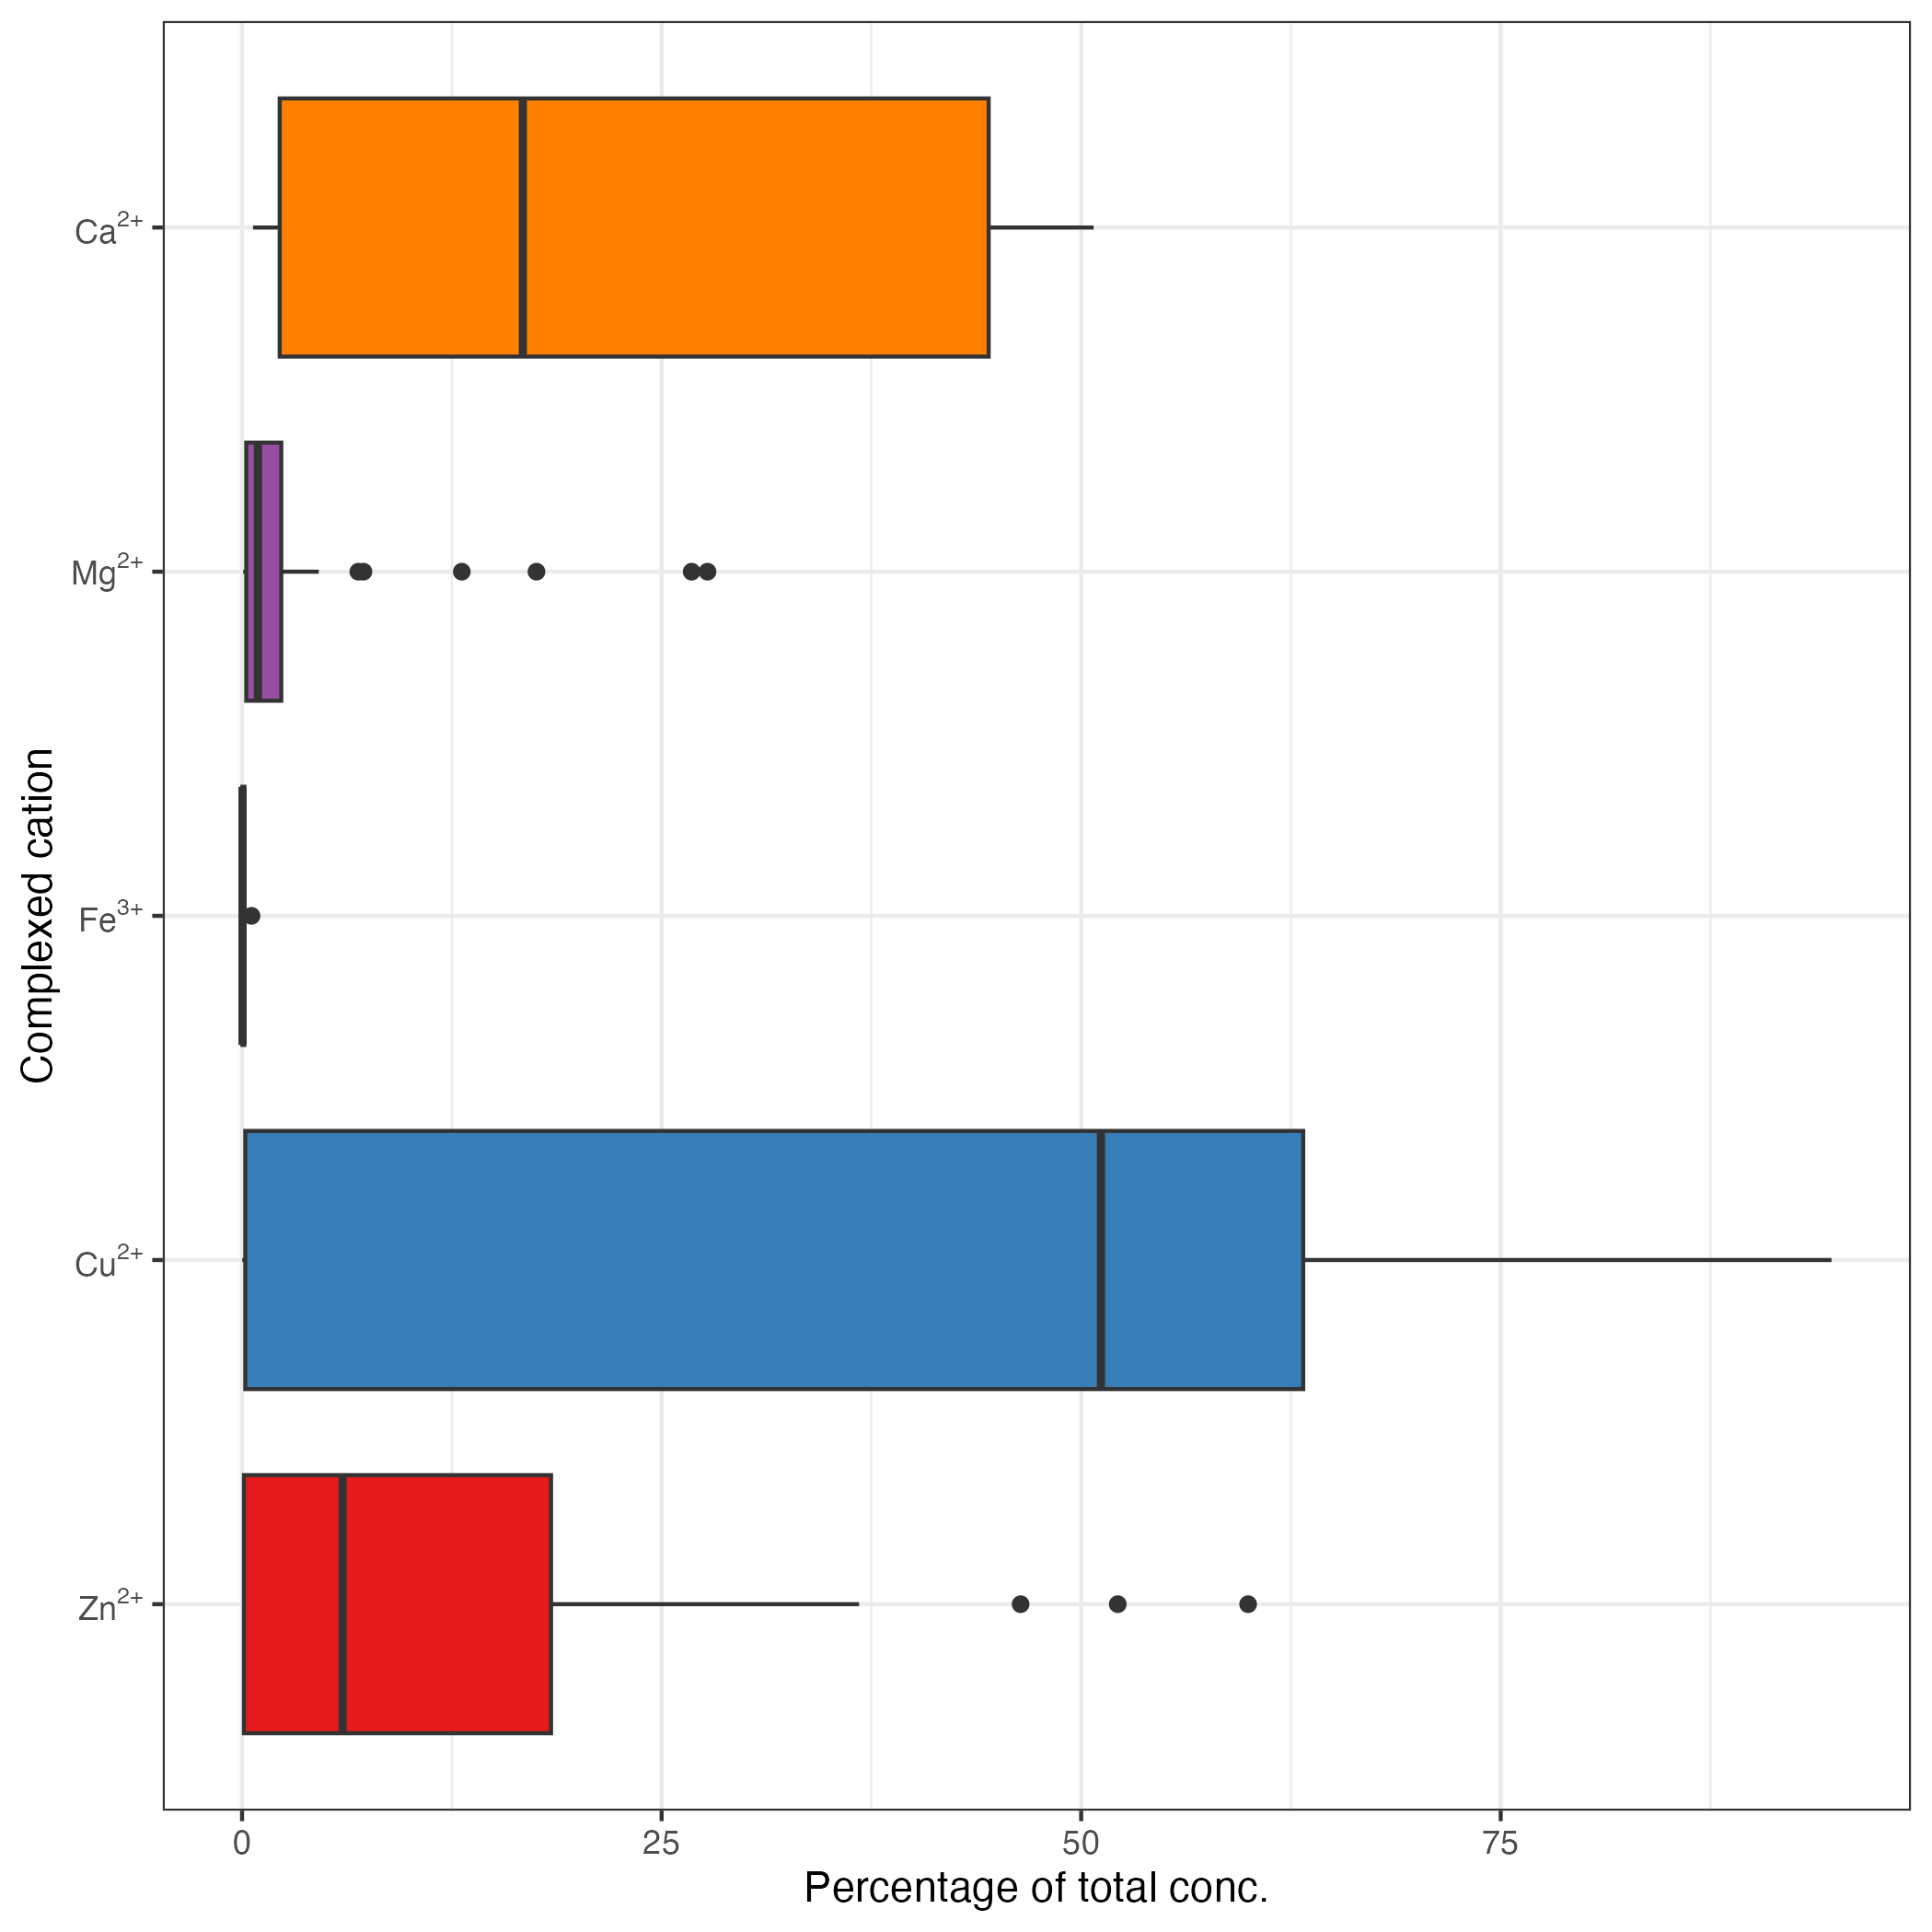
\includegraphics{plots/boxplot_species_dom_vm.png}
\caption{Complexation of cationic plant nutrients by DOM. Shown is the complexated proportion relative to the total concentration of the affected cationic plant nutrients in solution. Cation concentrations are derived from selected aquaponic studies (n = XXX). Calculations were made using Visual MINTEQ (Gaussian DOM) under the assumption that \(20 \text{ mg L}^{-1}\) of DOM are present in each system.}
\end{figure}

After determination of the proportion of plant nutrients masked by complexation, making them unavailable for precipitation, mineral saturation indices were calculated. This was to assess whether the solubility of a plant nutrient is controlled by the formation of precipitates, thus not enabling further dissolution. \textbf{FIGURE XXX} visualises the results, showing calculated \(\log(\frac{Q}{K})\) values for cationic plant nutrients with the corresponding precipitate-forming anions.

\begin{figure}
\centering
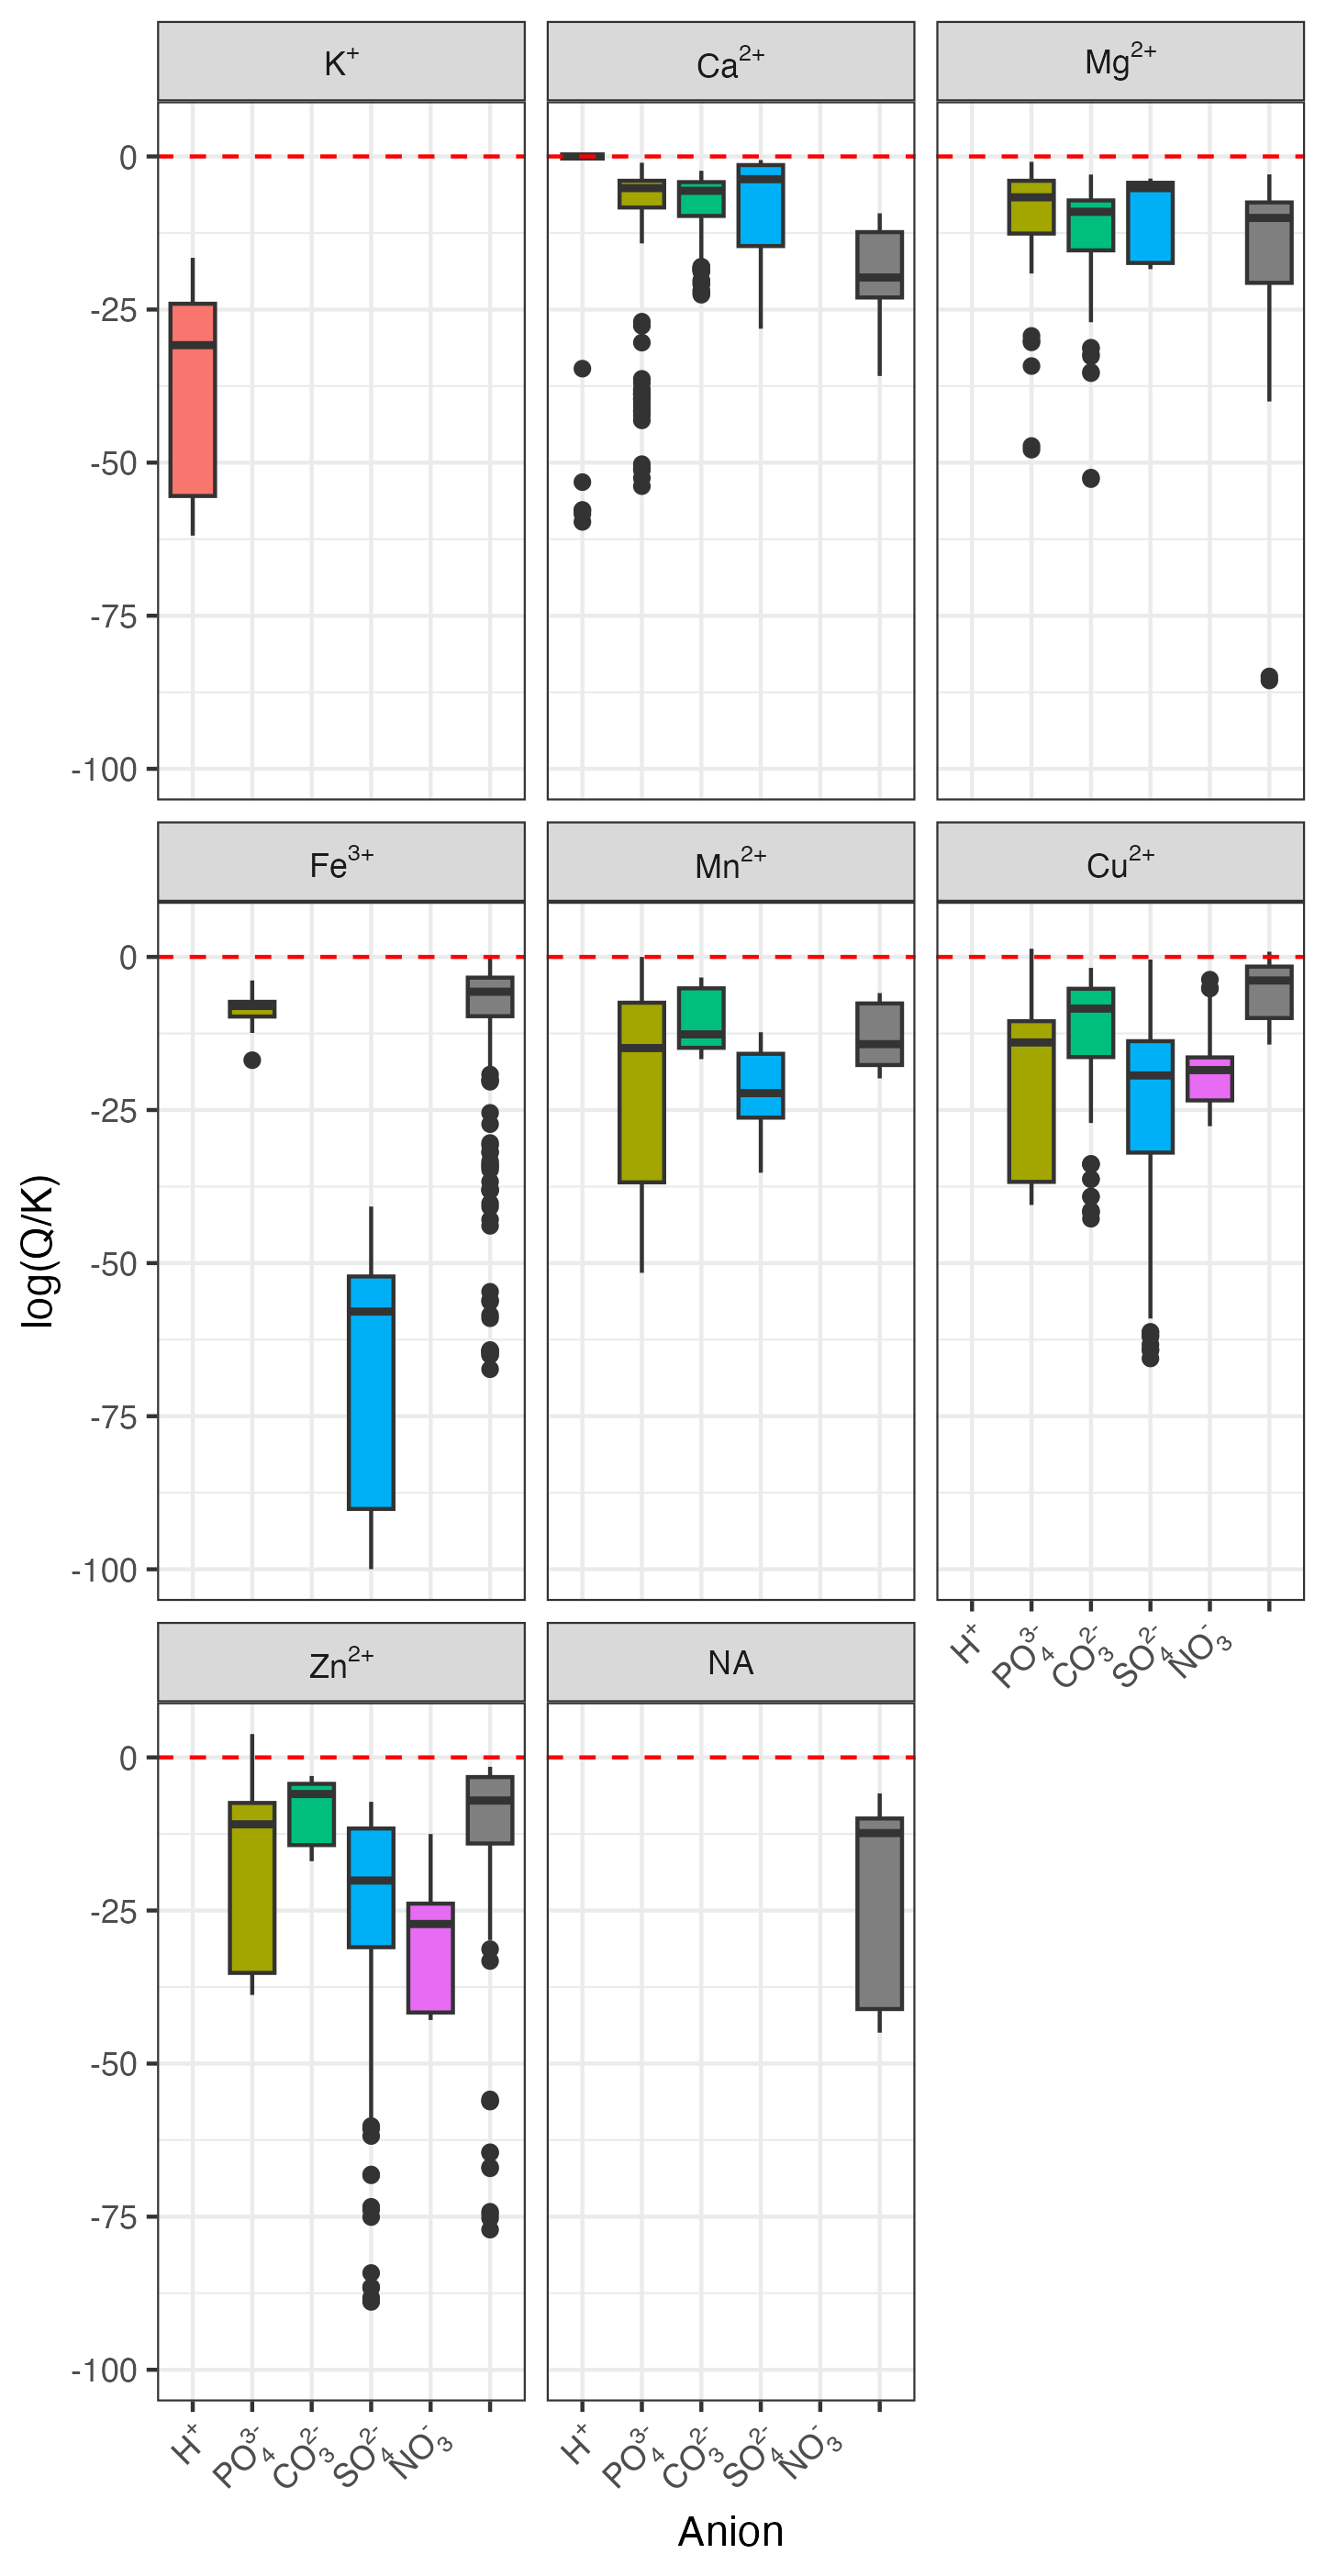
\includegraphics{plots/boxplot_empirical_saturation_vm.png}
\caption{Boxplot of mineral saturation indices of cations in relation to different anions calculated from aquaponic studies. Dashed red line describes 100\% saturation. Observations above the line indicate over-, those below the line undersaturation. Observations below but close to zero indicate solubility control by formation of a precipitate by the corresponding cation-anion combination.}
\end{figure}

The results indicate that maximum solubility of Ca, Fe and Cu was reached in several studies. In this context, the solubility of Ca appears to be controlled by the formation of carbonates due to the proximity of the \(\log(\frac{Q}{K})\) values to zero. The formation of phosphates was found to control the solubility of Fe, while both oxide and hydroxide formation determined the solubility of Cu. The solubility of Mn cannot be explained by the formation of precipitates and was thus likely controlled by formation of complex molecules. Zn solubility might have been controlled by the formation of carbonates and phosphates in few cases. However, the 75\% quantile value of the saturation index of -1.73 and -2.45 for carbonates and phosphates, respectively, indicates that the maximum concentration was not reached. Instead, the true concentration reached only \(10^{-1.73} \cdot 100\%\) = 1.86\% of the maximum saturation.

Those plant nutrients that were affected by precipitation were tested for the proportion of their total concentration that is expected to precipitate. The distribution of the obtained results is clearly bimodal as visible in \textbf{FIGURE XXX}. The median will thus be used in the following.

Overall, the plant nutrient that is affected most by precipitation was \(\text{PO}_{4}^{3-}\). Within the reviewed dataset, the median of the calculated percentage precipitation was \(98.0\%\), meaning that in 50\% of the studies more than \(98.0\%\) of \(\text{PO}_{4}^{3-}\) precipitated. On the other hand, in 12\% of the studies \(\text{PO}_{4}^{3-}\) precipitation was found not to occur at all.
A similar picture was observable for \(\text{Fe}^{3+}\). Here, no precipitation was expected to take place in \(45\%\) of the observations. However, in all other cases, \(\approx100\%\) of \(\text{Fe}^{3+}\) was predicted to precipitate.
Much less prone for precipitation were \(\text{Ca}^{2+}\), \(\text{Cu}^{2+}\) and \(\text{Mn}^{2+}\). Here, the median percentage precipitation was \(5.2\%\) in case of \(\text{Ca}^{2+}\), and \(0.0\%\) in case of \(\text{Cu}^{2+}\) and \(\text{Mn}^{2+}\), respectively.

\begin{figure}
\centering
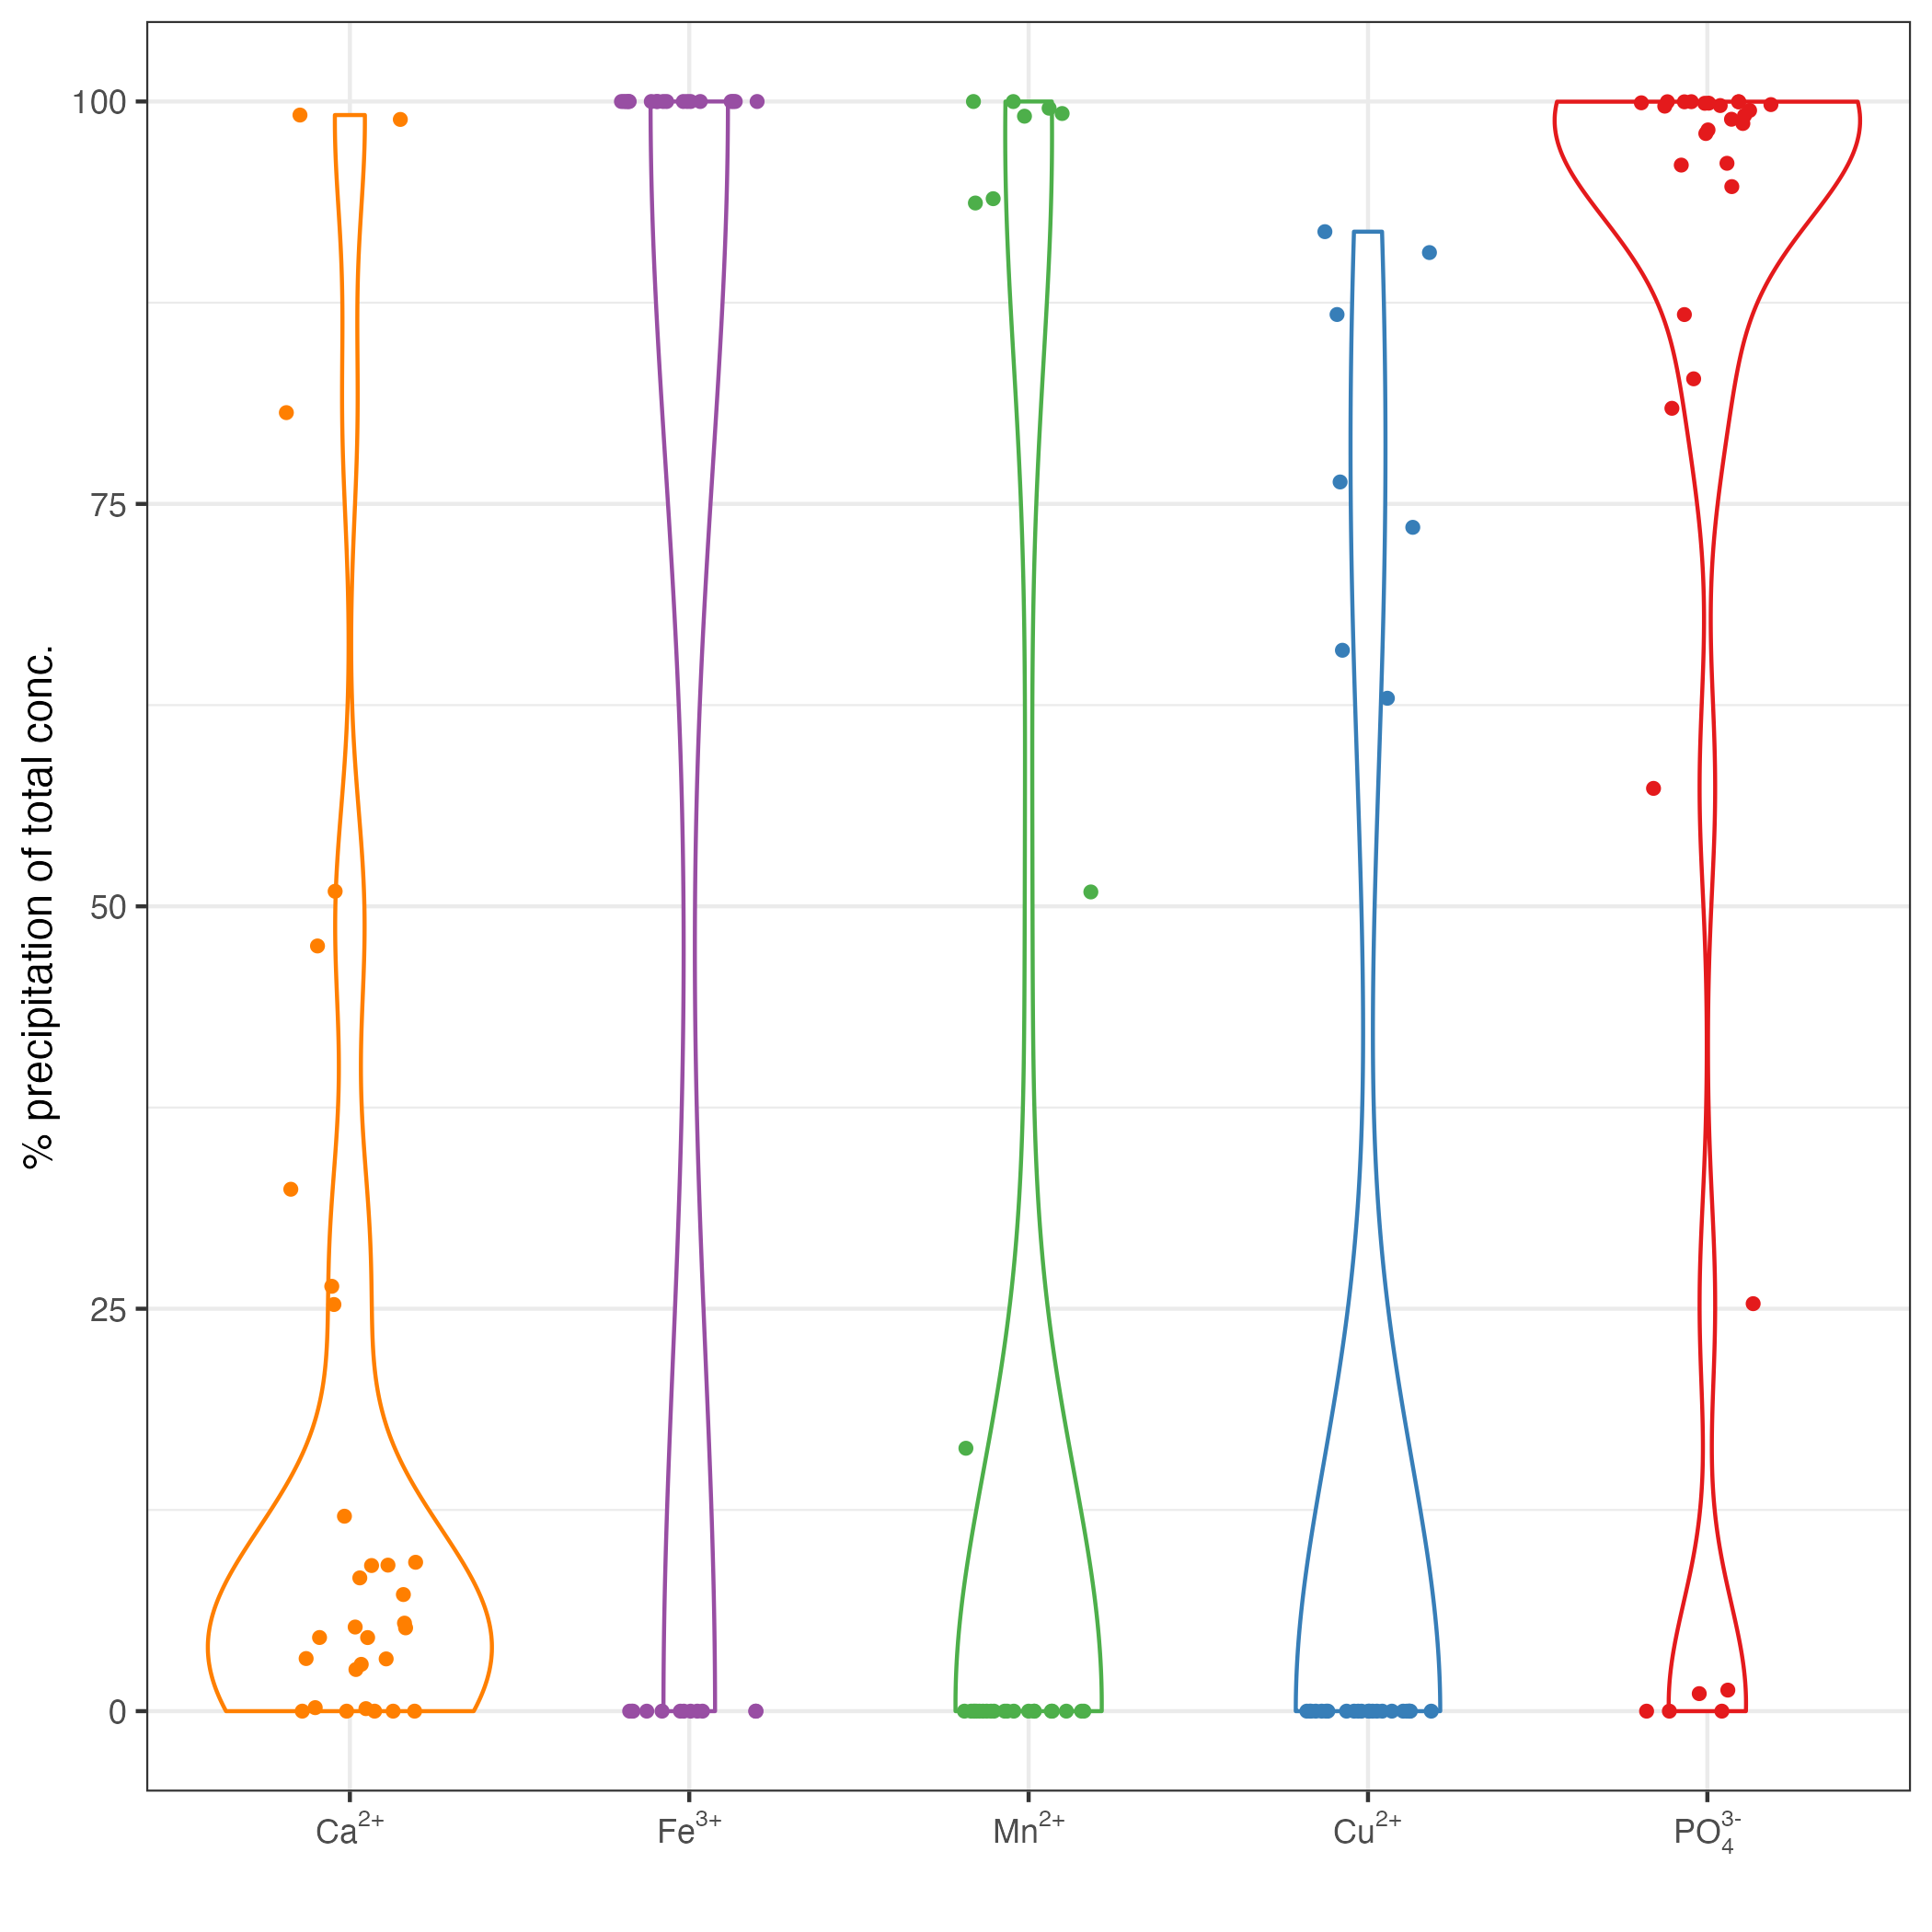
\includegraphics{plots/violinplot_precipitated2_vm.png}
\caption{Percentage of total amounts of plant nutrients present in solution that is prone to precipitation. Data originating from n = XXX publications.}
\end{figure}

\hypertarget{discussion}{%
\section{Discussion}\label{discussion}}

\hypertarget{sources-of-nutrients}{%
\subsection{Sources of nutrients}\label{sources-of-nutrients}}

The contribution of different nutrient sources to the total daily nutrient inputs into an aquaponic system were compared based on assumptions derived from literature.
Overall, the current input scenario confirms that fish feed is the major nutrient input route. Though, the results reveal that the source water is contributing an average of 50\% of the total Na input, 30\% of the Ca, 40\% of Mg and 30\% of S. Considering that salinity stress, ergo high Na concentrations, are toxic for most plants (Wu 2018), it is desirable to limit the influx into the system.
In the following, the assumptions are discussed. The average stocking density of 12.4 kg m\(^{-3}\) that was used for the nutrient contribution calculations can be considered representative for the intensive cultivation of \emph{Oreochromis} spp. (El-Sayed, 2019).
This is different for \emph{Clarias gariepinus}. The latter can be cultivated at stocking densities that are approximately ten times higher (\textasciitilde120 kg m\(^{-3}\)) without any adverse effects on fish health (Nieuwegiessen et al. 2009).
\emph{Sander lucioperca} is a species for which low stocking densities (\textasciitilde5 kg m\(^{-3}\)) are recommended (Kestemont, Dabrowski, and Summerfelt 2015).
Even though salmonids such as \emph{Oncorhynchus mykiss} are seldom reared in aquaponic systems, they can tolerate stocking densities up to 137 kg m\(^{-3}\). Though, normal stocking densities range between 10 and 20 kg m\(^{-3}\). The assumptions are rather on the lower end for salmonids (Pennell and McLean 1996).
\emph{Cyprinus carpio} is an irrelevant species for aquaponic systems due to its low market price. Though, it was found that fish welfare can be guaranteed at a stocking density of around 28 kg m\(^{-3}\), which is 2.3 times higher than the assumed density (Ruane, Carballo, and Komen 2002).
It can thus be expected that the contribution of feed to the total daily nutrient input in case of \emph{C. gariepinus} and \emph{C. carpio} is considerably higher than assumed due to rearing conditions in the reviewed studies that are not representative for production at commercial scale. In contrast, the assumptions might lead to an overestimation of the contribution of aquafeeds if \emph{S. lucioperca} is the species of choice.
Another aspect with respect to the contribution of feeds is that the feed composition is variable, depending on the selected species. Crude protein inclusion rates in commercial aquafeeds for the mentioned species range from \(32\%\) for \emph{C. carpio} (Wilson 2002) to \(50\%\) for percids (Geay and Kestemont 2015).

The current input scenarios are

The current input scenario lacks the consideration of the water removal step during the water exchange. This might, in reality, lead to a dilution of the nutrients if the concentrations in the system are higher than those in the source water. On the other hand, the source water could be a real addition of nutrients to the system if the concentration of nutrients in the system would drop below the concentration in the source water. This could, for instance, be the case due to plant uptake or other means of nutrient removal from the water column.
The total nutrient input calculations are therefore only valid if there is no nutrient loss through the removal of water but instead full retention of all nutrients within the system. This could be possible in systems where only evaporated water is refilled. However, such a scenario would come with a much lower water input rate than currently assumed.

\hypertarget{fate-and-behavior-of-nutrients-2}{%
\subsection{Fate and behavior of nutrients}\label{fate-and-behavior-of-nutrients-2}}

Nutrient imbalances are mentioned as causative factor for inconsistent performance of aquaponic systems. It was thus intended to pinpoint whether those imbalances occur due to lacking supply or due to physico-chemical constraints that are controlling the maximum concentration of the affecteed nutrients. Considering that aquaponic systems contain DOM, complexation percentages of plant nutrients by DOM were calculated to identify the proportion of plant nutrients available for precipitation reactions. Saturation indices were eventually calculated to identify saturated nutrients. Those were finally assessed with respect to the percentage saturation to find out what proportion of these nutrients might remain in solution.
The limitations of Ca, Fe and Cu that were found in the scope of this study are in line with previous publications {[}Goddek et al. (2015); Bittsanszky2016{]}. Empirical studies intending to manipulate the concentrations of these compounds by increasing their inclusion rate into aquafeeds could not find an effect (Seawright, Stickney, and Walker 1998).

that could not find an increase in the concentration of these compounds in solution if the feed inclusion rate was increased (Shaw, Seawright). Nutrient imbalances appear thus to be a result of chemical constraints. It can be further hypothetised that reported nutrient losses are due to the formation of precipitates in the system (Delaide et al. 2017). If precipitation occurs in inaccessible places such as the inside of pipes or other surfaces, these nutrients will not be taken into account when analysing, for instace, sludge samples. The nutrients would, however, not be lost but instead they are deposited out of reach.
On the other hand, considering the positive saturation index values that were found for Fe and Mn, it is likely that other factors are controlling their solubility. Both ions might be kept in solution due to organic matter that is a natural ligand, forming chelates. However, this would lead to an increase in dissolved phosphate that might eventually form precipitates with other compounds or could be taken up by plants.

\hypertarget{implications-for-the-formulation-of-tailored-aquaponics-feeds}{%
\subsection{Implications for the formulation of tailored aquaponics feeds}\label{implications-for-the-formulation-of-tailored-aquaponics-feeds}}

The formulation of a dedicated aquaponics feed is seen as potentially user-friendly and rapid way of adding nutrients to the system, resulting in close-to optimum concentrations for the plants.

It is reasonable to focus on well-soluble nutrients that were not found to be constrained by precipitation reactions. Potential candidates that are fulfilling these requirements are alkaline metals such as K. The solubility of salts containing K is usually within the range of several grams per liter. Losses of K due to the formation of precipitates is thus unlikely. Other studies confirmed that the concentration of K in solution can be altered by different inclusion rates of K (Seawright, Stickney, and Walker 1998; Shaw, Knopf, and Kloas 2022). The same was also suggested by the nutrient release coefficient concept that was recently suggested (\textbf{Cerozi2022?}).
However, considering the contribution of feed in comparison to the contribution of KOH, if used for pH management, it is questionable what makes more sense

Another alkaline metal that is of interest with respect to aquapfeeds tailored for aquaponics is Na.

Explicitly considering an increased delivery of plant nutrients other than K might be counterproductive, considering the potential precipitation of these nutrients.

\hypertarget{implications-for-the-management-of-aquaponic-systems}{%
\subsection{Implications for the management of aquaponic systems}\label{implications-for-the-management-of-aquaponic-systems}}

In general, lowering the pH in the aquaculture unit would mobilize nutrients. Even though it is reported that the activity of nitrifyers is impaired under acidic conditions, it was also found that there are

\hypertarget{future-research-needs}{%
\subsection{Future research needs}\label{future-research-needs}}

Aquaponics is an interdisciplinary field, combining both aquaculture and horticulture but also aquatic chemistry. The implications arising from chemistry are, however, not examined. Data is lacking as even studies dedicated to nutrient cycling in aquaponics are not following best practices with respect to reporting of analytical results, with lacking standard deviations, lacking detection and quantification limits of their methods and alike.
With respect to more accurate data, usually only averaged nutrient concentrations are reported, while the evolution of nutrient concentrations over time is of greater interest due to the kinetics of certain reactions.
In terms of chemical modeling, temperatures, and pH values
It is, however, necessary to understand the chemistry of aquaponic systems.

Furthermore, there is no published study that is assessing the effects of organic matter in aquaponic systems. Besides pH, the key difference between aquaponic and hydroponic systems is the concentration of organic matter in the water. Organic matter is the main chelating agent and main factor affecting the mobility of metals. Water from aquaculture is much richer in organic matter than natural waters. Its effects should therefore be assessed.

Lastly, it is questionable whether the total concentration of the nutrients is actually of importance for plants. It was reported that a reduction of macronutrient concentrations to 50\% of the control level does not have no adverse effect on growth, fruit yield and fruit quality in tomato (Siddiqi et al., 1998). The stoichiometry of nutrient solutions might thus play a more vital role for plants than currently known.

\hypertarget{references}{%
\section*{References}\label{references}}
\addcontentsline{toc}{section}{References}

\hypertarget{refs}{}
\begin{CSLReferences}{1}{0}
\leavevmode\vadjust pre{\hypertarget{ref-Bittsanszky2016}{}}%
Bittsánszky, András, Nikolett Uzinger, Gábor Gyulai, Alex Mathis, Ranka Junge, Morris Villarroel, Benzion Kotzen, and Tamás Kőmı́ves. 2016. {``Nutrient Supply of Plants in Aquaponic Systems.''} \emph{Ecocycles} 2 (2). \url{https://doi.org/10.19040/ecocycles.v2i2.57}.

\leavevmode\vadjust pre{\hypertarget{ref-Bury2003}{}}%
Bury, Nicolas R., Paul A. Walker, and Chris N. Glover. 2003. {``Nutritive Metal Uptake in Teleost Fish.''} \emph{Journal of Experimental Biology} 206 (1): 11--23. \url{https://doi.org/10.1242/jeb.00068}.

\leavevmode\vadjust pre{\hypertarget{ref-EU2020}{}}%
Council of the European Union. 2020. {``{Council Directive 98/83/EC of 3 November 1998 on the quality of water intended for human consumption}.''}

\leavevmode\vadjust pre{\hypertarget{ref-Dabrowski2002}{}}%
Dabrowski, Konrad, and Helga Guderley. 2002. {``{Intermediary Metabolism}.''} In \emph{Fish Nutrition}, Third, 309--65. Elsevier Science.

\leavevmode\vadjust pre{\hypertarget{ref-DeRijck1999b}{}}%
De Rijck, G., and E. Schrevens. 1999b. {``Chemical Feasibility Region for Nutrient Solutions in Hydroponic Plant Nutrition.''} \emph{Journal of Plant Nutrition} 22 (2): 259--68.

\leavevmode\vadjust pre{\hypertarget{ref-DeRijck1997}{}}%
---------. 1997. {``pH Influenced by the Elemental Composition of Nutrient Solutions.''} \emph{Journal of Plant Nutrition} 20 (7 \& 8): 911--23.

\leavevmode\vadjust pre{\hypertarget{ref-DeRijck1998a}{}}%
---------. 1998a. {``Comparison of the Mineral Composition of Twelve Standard Nutrient Solutions.''} \emph{Journal of Plant Nutrition} 21 (10): 2115--25.

\leavevmode\vadjust pre{\hypertarget{ref-DeRijck1998}{}}%
---------. 1998b. {``Elemental Bioavailability in Nutrient Solutions in Relation to Complexation Reactions.''} \emph{Journal of Plant Nutrition} 21 (5): 849--59.

\leavevmode\vadjust pre{\hypertarget{ref-Delaide2017}{}}%
Delaide, Boris, Guillaume Delhaye, Michael Dermience, James Gott, Hélène Soyeurt, and M. Haissam Jijakli. 2017. {``Plant and Fish Production Performance, Nutrient Mass Balances, Energy and Water Use of the {PAFF} Box, a Small-Scale Aquaponic System.''} \emph{Aquacultural Engineering} 78: 130--39. \url{https://doi.org/10.1016/j.aquaeng.2017.06.002}.

\leavevmode\vadjust pre{\hypertarget{ref-Delaide2016}{}}%
Delaide, Boris, Simon Goddek, James Gott, Hélène Soyeurt, and M. Jijakli. 2016. {``{Lettuce (\emph{Lactuca sativa} L. var. Sucrine) Growth Performance in Complemented Aquaponic Solution Outperforms Hydroponics}.''} \emph{Water} 8 (10): 467. \url{https://doi.org/10.3390/w8100467}.

\leavevmode\vadjust pre{\hypertarget{ref-DIN32645}{}}%
Deutsches Institut für Normung e.V. 2008. \emph{{Chemical analysis - Decision limit, detection limit and determination limit under repeatability conditions - Terms, methods, evaluation}}. DIN 32645:2008-11. Beuth Verlag {GmbH}. \url{https://doi.org/10.31030/1465413}.

\leavevmode\vadjust pre{\hypertarget{ref-Eck2019}{}}%
Eck, Mathilde, Oliver Körner, and M. Haïssam Jijakli. 2019. {``{Nutrient Cycling in Aquaponics Systems}.''} In \emph{Aquaponics Food Production Systems}, 231--46. Springer International Publishing. \url{https://doi.org/10.1007/978-3-030-15943-6_9}.

\leavevmode\vadjust pre{\hypertarget{ref-Geay2015}{}}%
Geay, Florian, and Patrick Kestemont. 2015. {``Feeding and Nutrition of Percid Fishes During Ongrowing Stages.''} In \emph{Biology and Culture of Percid Fishes}, 587--622. Springer Netherlands. \url{https://doi.org/10.1007/978-94-017-7227-3_22}.

\leavevmode\vadjust pre{\hypertarget{ref-Goddek2015}{}}%
Goddek, Simon, Boris Delaide, Utra Mankasingh, Kristin Ragnarsdottir, Haissam Jijakli, and Ragnheidur Thorarinsdottir. 2015. {``{Challenges of Sustainable and Commercial Aquaponics}.''} \emph{Sustainability} 7 (4): 4199--4224. \url{https://doi.org/10.3390/su7044199}.

\leavevmode\vadjust pre{\hypertarget{ref-Grimm1991}{}}%
Grimm, David M., Leo V. Azarraga, Lionel A. Carreira, and Wisnu Susetyo. 1991. {``{Continuous Multiligand Distribution Model Used To Predict the Stability Constant of Cu(II) Metal Complexation with Humic Material from Fluorescence Quenching Data}.''} \emph{Environmental Science and Technology} 25: 1427--31.

\leavevmode\vadjust pre{\hypertarget{ref-Guillaume2001}{}}%
Guillaume, Jean, Sadasivam Kaushik, Pierre Bergot, and Robert Metailler. 2001. \emph{Nutrition and Feeding of Fish and Crustaceans (Springer Praxis Books / Food Sciences)}. Springer.

\leavevmode\vadjust pre{\hypertarget{ref-Hardy2002}{}}%
Hardy, Ronald. 2002. \emph{Fish Nutrition}. Elsevier Science \& Technology Books.

\leavevmode\vadjust pre{\hypertarget{ref-IAFFD2021}{}}%
International Aquaculture Feed Formulation Database (IAFFD). 2021. {``{Feed Ingredients Composition Database (FICD) v7.0}.''} \url{https://app.iaffd.com}.

\leavevmode\vadjust pre{\hypertarget{ref-Jensen2003}{}}%
Jensen, James N. 2003. \emph{A Problem-Solving Approach to Aquatic Chemistry}. 1\^{}st ed. Wiley.

\leavevmode\vadjust pre{\hypertarget{ref-Joyce2019}{}}%
Joyce, Alyssa, Mike Timmons, Simon Goddek, and Timea Pentz. 2019. {``{Bacterial Relationships in Aquaponics: New Research Directions}.''} In \emph{Aquaponics Food Production Systems}, 145--61. Springer International Publishing. \url{https://doi.org/10.1007/978-3-030-15943-6_6}.

\leavevmode\vadjust pre{\hypertarget{ref-Kestemont2015}{}}%
Kestemont, Patrick, Konrad Dabrowski, and Robert C. Summerfelt, eds. 2015. {``Biology and Culture of Percid Fishes.''} \url{https://doi.org/10.1007/978-94-017-7227-3}.

\leavevmode\vadjust pre{\hypertarget{ref-Kloas2015}{}}%
Kloas, W, R Groß, D Baganz, J Graupner, H Monsees, U Schmidt, G Staaks, et al. 2015. {``A New Concept for Aquaponic Systems to Improve Sustainability, Increase Productivity, and Reduce Environmental Impacts.''} \emph{Aquaculture Environment Interactions} 7 (2): 179--92. \url{https://doi.org/10.3354/aei00146}.

\leavevmode\vadjust pre{\hypertarget{ref-Lall2002}{}}%
Lall, Santosh P. 2002. {``{The Minerals}.''} In \emph{Fish Nutrition}, Third, 259--308. Elsevier Science.

\leavevmode\vadjust pre{\hypertarget{ref-Lennard2019}{}}%
Lennard, Wilson, and Simon Goddek. 2019. {``{Aquaponics: The Basics}.''} In \emph{Aquaponics Food Production Systems}, 113--43. Springer International Publishing. \url{https://doi.org/10.1007/978-3-030-15943-6_5}.

\leavevmode\vadjust pre{\hypertarget{ref-Lunda2019}{}}%
Lunda, Roman, Koushik Roy, Jan Másı́lko, and Jan Mráz. 2019. {``Understanding Nutrient Throughput of Operational {RAS} Farm Effluents to Support Semi-Commercial Aquaponics: Easy Upgrade Possible Beyond Controversies.''} \emph{Journal of Environmental Management} 245: 255--63. \url{https://doi.org/10.1016/j.jenvman.2019.05.130}.

\leavevmode\vadjust pre{\hypertarget{ref-Maathuis2014}{}}%
Maathuis, Frans J. M., Izhar Ahmad, and Juan Patishtan. 2014. {``Regulation of Na\(\mathplus\) Fluxes in Plants.''} \emph{Frontiers in Plant Science} 5 (September). \url{https://doi.org/10.3389/fpls.2014.00467}.

\leavevmode\vadjust pre{\hypertarget{ref-Marschner2012}{}}%
Marschner, Petra, ed. 2012. \emph{Marschner's Mineral Nutrition of Higher Plants}. 3rd ed. Academic Press. \url{https://www.ebook.de/de/product/14765252/marschner_s_mineral_nutrition_of_higher_plants.html}.

\leavevmode\vadjust pre{\hypertarget{ref-Maucieri2019a}{}}%
Maucieri, Carmelo, Carlo Nicoletto, Giampaolo Zanin, Marco Birolo, Angela Trocino, Paolo Sambo, Maurizio Borin, and Gerolamo Xiccato. 2019. {``Effect of Stocking Density of Fish on Water Quality and Growth Performance of European Carp and Leafy Vegetables in a Low-Tech Aquaponic System.''} Edited by Jay Richard Stauffer. \emph{{PLOS} {ONE}} 14 (5): e0217561. \url{https://doi.org/10.1371/journal.pone.0217561}.

\leavevmode\vadjust pre{\hypertarget{ref-Mengel2001}{}}%
Mengel, Konrad, Ernest A. Kirkby, Harald Kosegarten, and Thomas Appel, eds. 2001. {``Principles of Plant Nutrition.''} \url{https://doi.org/10.1007/978-94-010-1009-2}.

\leavevmode\vadjust pre{\hypertarget{ref-Monsees2019}{}}%
Monsees, Hendrik, Johanna Suhl, Maurice Paul, Werner Kloas, Dennis Dannehl, and Sven Würtz. 2019. {``Lettuce (Lactuca Sativa, Variety Salanova) Production in Decoupled Aquaponic Systems: Same Yield and Similar Quality as in Conventional Hydroponic Systems but Drastically Reduced Greenhouse Gas Emissions by Saving Inorganic Fertilizer.''} Edited by Rafiq Islam. \emph{{PLOS} {ONE}} 14 (6): e0218368. \url{https://doi.org/10.1371/journal.pone.0218368}.

\leavevmode\vadjust pre{\hypertarget{ref-Nieuwegiessen2009}{}}%
Nieuwegiessen, Pascal G. van de, Jacob Olwo, Sophoan Khong, Johan A. J. Verreth, and Johan W. Schrama. 2009. {``Effects of Age and Stocking Density on the Welfare of African Catfish, Clarias Gariepinus Burchell.''} \emph{Aquaculture} 288 (1-2): 69--75. \url{https://doi.org/10.1016/j.aquaculture.2008.11.009}.

\leavevmode\vadjust pre{\hypertarget{ref-Oikari1985}{}}%
Oikari, A. O., and J. C. Rankin. 1985. {``Renal Excretion of Magnesium in a Freshwater Teleost, \emph{Salmo Gairdneri}.''} \emph{Journal of Experimental Biology} 117 (1): 319--33. \url{https://doi.org/10.1242/jeb.117.1.319}.

\leavevmode\vadjust pre{\hypertarget{ref-Pantanella2012}{}}%
Pantanella, E., M. Cardarelli, G. Colla, E. Rea, and A. Marucci. 2012. {``Aquaponics Vs. Hydroponics: Production and Quality of Lettuce Crop.''} Edited by N. Castilla, S. Sase, W. H. Schnitzler, O. van Kooten, J. F. Meneses, and E. van Oos.

\leavevmode\vadjust pre{\hypertarget{ref-Pennell1996}{}}%
Pennell, William, and William E. McLean. 1996. {``Early Rearing.''} In \emph{Principles of Salmonid Culture}, edited by William Pennell and Bruce A. Barton, 365--465. Elsevier B.V.

\leavevmode\vadjust pre{\hypertarget{ref-Quagrainie2017}{}}%
Quagrainie, Kwamena K., Roberto Manolio Valladão Flores, Hye-Ji Kim, and Verena McClain. 2017. {``Economic Analysis of Aquaponics and Hydroponics Production in the u.s. Midwest.''} \emph{Journal of Applied Aquaculture} 30 (1): 1--14. \url{https://doi.org/10.1080/10454438.2017.1414009}.

\leavevmode\vadjust pre{\hypertarget{ref-Rakocy2006}{}}%
Rakocy, James E., Michael P. Masser, and Thomas M. Losordo. 2006. {``Recirculating Aquaculture Tank Production Systems: Aquaponics - Integrating Fish and Plant Culture.''} In \emph{Southern Regional Aquaculture Center (SRAC) Publications}. Vol. 454. Oklahoma State University.

\leavevmode\vadjust pre{\hypertarget{ref-Resh2016}{}}%
Resh, Howard M. 2016. \emph{{Hydroponic Food Production}}. Taylor \& Francis Ltd. \url{https://www.ebook.de/de/product/21177729/howard_m_resh_hydroponic_food_production.html}.

\leavevmode\vadjust pre{\hypertarget{ref-Robaina2019}{}}%
Robaina, Lidia, Juhani Pirhonen, Elena Mente, Javier Sánchez, and Neill Goosen. 2019. {``{Fish Diets in Aquaponics}.''} In \emph{Aquaponics Food Production Systems}, 333--52. Springer International Publishing. \url{https://doi.org/10.1007/978-3-030-15943-6_13}.

\leavevmode\vadjust pre{\hypertarget{ref-Rodgers2022}{}}%
Rodgers, Dylan, Eugene Won, Michael B. Timmons, and Neil Mattson. 2022. {``Complementary Nutrients in Decoupled Aquaponics Enhance Basil Performance.''} \emph{Horticulturae} 8 (2): 111. \url{https://doi.org/10.3390/horticulturae8020111}.

\leavevmode\vadjust pre{\hypertarget{ref-Ruane2002}{}}%
Ruane, N. M., E. C. Carballo, and J. Komen. 2002. {``{Increased stockin g densit y influences the acute p h y siolo g ical stress res p onse of common carp \emph{Cyprinus carpio} ( L.)}.''} \emph{Aquaculture Research} 33: 777--84.

\leavevmode\vadjust pre{\hypertarget{ref-Sambo2019}{}}%
Sambo, Paolo, Carlo Nicoletto, Andrea Giro, Youry Pii, Fabio Valentinuzzi, Tanja Mimmo, Paolo Lugli, et al. 2019. {``Hydroponic Solutions for Soilless Production Systems: Issues and Opportunities in a Smart Agriculture Perspective.''} \emph{Frontiers in Plant Science} 10 (923): 1--17. \url{https://doi.org/10.3389/fpls.2019.00923}.

\leavevmode\vadjust pre{\hypertarget{ref-Seawright1998}{}}%
Seawright, Damon E., Robert R. Stickney, and Richard B. Walker. 1998. {``Nutrient Dynamics in Integrated Aquaculture-Hydroponics Systems.''} \emph{Aquaculture} 160: 215--37.

\leavevmode\vadjust pre{\hypertarget{ref-Shaw2022}{}}%
Shaw, Christopher, Klaus Knopf, and Werner Kloas. 2022. {``Fish Feeds in Aquaponics and Beyond: A Novel Concept to Evaluate Protein Sources in Diets for Circular Multitrophic Food Production Systems.''} \emph{Sustainability} 14 (7): 4064. \url{https://doi.org/10.3390/su14074064}.

\leavevmode\vadjust pre{\hypertarget{ref-Stumm1981}{}}%
Stumm, Werner. 1981. \emph{Aquatic Chemistry: Chemical Equilibria and Rates in Natural Waters}. 3rd ed. Wiley.

\leavevmode\vadjust pre{\hypertarget{ref-Sugiura2018}{}}%
Sugiura, Shozo H. 2018. {``Phosphorus, Aquaculture, and the Environment.''} \emph{Reviews in Fisheries Science {\&}Amp\(\mathsemicolon\) Aquaculture} 26 (4): 515--21. \url{https://doi.org/10.1080/23308249.2018.1471040}.

\leavevmode\vadjust pre{\hypertarget{ref-Sugiura1998}{}}%
Sugiura, Shozo H., Faye M. Dong, Cindra K. Rathbone, and Ronald W. Hardy. 1998. {``Apparent Protein Digestibility and Mineral Availabilities in Various Feed Ingredients for Salmonid Feeds.''} \emph{Aquaculture} 159: 177--202.

\leavevmode\vadjust pre{\hypertarget{ref-Tacon1983}{}}%
Tacon, Albert G. J., and S. S. de Silva. 1983. {``{Mineral composition of some commercial fish feeds available in Europe}.''} \emph{Aquaculture} 31: 11--20.

\leavevmode\vadjust pre{\hypertarget{ref-Timmons2010}{}}%
Timmons, M. B. 2010. \emph{Recirculating Aquaculture: 2nd Edition}. Cayuga Aqua Ventures.

\leavevmode\vadjust pre{\hypertarget{ref-Turnsek2020}{}}%
Turnsek, Maja, Agnes Joly, Ragnheidur Thorarinsdottir, and Ranka Junge. 2020. {``Challenges of Commercial Aquaponics in Europe: Beyond the Hype.''} \emph{Water} 12 (1): 306. \url{https://doi.org/10.3390/w12010306}.

\leavevmode\vadjust pre{\hypertarget{ref-Ward2011}{}}%
Ward, Bess B., D. J. Arp, and Martin G. Klotz. 2011. \emph{Nitrification}. ASM Press.

\leavevmode\vadjust pre{\hypertarget{ref-Wilson2002}{}}%
Wilson, Robert P. 2002. {``{Amino Acids and Proteins}.''} In \emph{Fish Nutrition}, Third, 143--79. Elsevier Science. \url{https://doi.org/10.1016/b978-012319652-1/50004-5}.

\leavevmode\vadjust pre{\hypertarget{ref-Wu2018}{}}%
Wu, Honghong. 2018. {``Plant Salt Tolerance and Na+ Sensing and Transport.''} \emph{The Crop Journal} 6 (3): 215--25. \url{https://doi.org/10.1016/j.cj.2018.01.003}.

\end{CSLReferences}

\end{document}
